
\documentclass[twoside,openright,titlepage,fleqn,pointlessnumbers,headinclude,,% 
                11pt,a4paper,BCOR5mm,footinclude,cleardoubleempty,abstracton % <--- obsolete, remove (todo)
                ]{scrreprt}
\listfiles

\newcommand{\myTitle}{Evolution of Heat Flow Prediction Models for FPGA Devices \xspace}
\newcommand{\mySubTitle}{\xspace}
\newcommand{\myDegree}{Bachelor of Science \xspace}
\newcommand{\myName}{Hendrik Hangmann \xspace}
\newcommand{\myAdress}{Giefersstrasse 7 \\33102 Paderborn\xspace}
\newcommand{\myNumber}{Matriculation number: 6533440\xspace}
\newcommand{\myProf}{Dr. Paul Kaufmann \xspace}
\newcommand{\myOtherProf}{Jun-Prof. Dr. Christian Plessl \xspace}
%\newcommand{\mySupervisor}{Dr. Paul Kaufmann \xspace}
\newcommand{\myFaculty}{	Faculty for Electrical Engineering, Computer Science and Mathematics \xspace}
\newcommand{\myDepartment}{	Department of Computer Science \xspace}
\newcommand{\myUni}{\protect{University of Paderborn}\xspace}
\newcommand{\myLocation}{Paderborn\xspace}
\newcommand{\myThesisType}{Masterthesis}
\newcommand{\myTime}{\today\xspace}
\newcommand{\myVersion}{Version 0.1\xspace}
%*******************************************************
% Packages with options that might require adjustments
%*******************************************************
\usepackage{amsfonts} 

\usepackage[latin1]{inputenc} %ggfs. auf andere Plattform anpassen
\usepackage[T1]{fontenc} 
\usepackage[american]{babel}           
%\usepackage{apalike} 
%\usepackage{natbib} 
\usepackage{framed}
 
%\usepackage{chapter}     
\usepackage[fleqn]{amsmath} % math environments and more by the AMS
\usepackage{setspace}
\usepackage{color}
	\definecolor{pantone536}{cmyk}{0.3,0.18,0.06,0}
	\definecolor{pantone428}{cmyk}{0,0,0,0.2}
	\definecolor{pantone5793}{cmyk}{0.06,0,0.23,0.18}
	\definecolor{pantone281}{cmyk}{1,0.72,0,0.38}
	\definecolor{pantone129}{cmyk}{0,0.15,0.76,0}
	\definecolor{pantone152}{cmyk}{0,0.51,1,0}
	\definecolor{pantone376}{cmyk}{0.56,0,1,0}
	
\usepackage{listings} 
\definecolor{orange}{rgb}{0.8,0.3,0.3}
\lstset{language=VHDL,
%   basicstyle=\scriptsize\ttfamily,
   keywordstyle=\color{blue},
   emph={square}, 
   emphstyle=\color{pantone536},
%   stringstyle=\color{green}\ttfamily,
   commentstyle=\color{middlegray}\ttfamily}
% basicstyle=\tiny\ttfamily}	
%*******************************************************
% todos
%*******************************************************
\newcounter{todozaehler}[chapter]
\setcounter{todozaehler}{0}
\renewcommand{\thetodozaehler}{\thechapter.\arabic{todozaehler}~}
\setcounter{todozaehler}{0}

\newcommand{\todo}[1]{{\refstepcounter{todozaehler}\graffito{\colorbox{pantone152}{\parbox{25mm}{\scriptsize\textcolor{white}{\textbf{\textsf{TODO \thetodozaehler}}}}} \colorbox{pantone152}{\parbox{25mm}{\raggedright\scriptsize\textcolor{white}{ \sf \em #1}}}}}}

%*******************************************************
\usepackage{classicthesis-ldpkg} 
%*******************************************************
% Options for classicthesis.sty:
% tocaligned eulerchapternumbers drafting linedheaders listsseparated
% subfig nochapters beramono eulermath parts minionpro pdfspacing
%\usepackage[drafting,pdfspacing,linedheaders,tocaligned,
 %           subfig,eulermath,parts,dottedtoc]{classicthesis}
\usepackage[pdfspacing,linedheaders,tocaligned,
            subfig,eulermath,parts,dottedtoc]{classicthesis}
\usepackage{subfig}
%*******************************************************
%ArsClassica changes some typographic settings in classicthesis
\usepackage[english]{arsclassica}
\usepackage[tight,american]{minitoc} 
	\def\ptctitle{inhaltsverzeichnis}
      \def\mtctitle{inhaltsverzeichnis}
      \def\stctitle{inhaltsverzeichnis}
      \setlength{\mtcindent}{0pt}
      \renewcommand{\mtifont}{\normalsize\sffamily%
         \scshape\lsstyle}
         \setcounter{minitocdepth}{1}
%\usepackage{showidx}
\usepackage{makeidx}                    
%*******************************************************
%*******************************************************            
%\usepackage[section,below]{placeins} <--- not everybody wants this
%\usepackage[all]{hypcap} <--- does not work with MiKTeX 2.6
% ********************************************************************
% Language/strings for backrefs (change here, thanks, Lorenzo)
%*******************************************************
%\renewcommand{\backrefnotcitedstring}{\relax}%(Not cited.)
%\renewcommand{\backrefcitedsinglestring}[1]{(Citato a pagina~#1.)}
%\renewcommand{\backrefcitedmultistring}[1]{(Citato alle pagine~#1.)}
%\renewcommand{\backreftwosep}{ e~}
%\renewcommand{\backreflastsep}{ e~}
% ********************************************************************
% Setup and Finetuning
%*******************************************************
\newlength{\abcd} % for ab..z string length calculation
\newcommand{\myfloatalign}{\centering} % how all the floats will be aligned
\setlength{\extrarowheight}{3pt} % increase table row height
\clubpenalty = 10000
\widowpenalty = 10000
\displaywidowpenalty = 10000
\parindent=0cm
\parskip=1ex     
\usepackage{blindtext}
\newtheorem{mydef}{Definition}
\usepackage{subfig}
% ********************************************************************
% Captions look and feel
%*******************************************************
\captionsetup{format=hang,font=small}
% ********************************************************************
% Where to look for graphics
%*******************************************************
%\graphicspath{{gfx/}{misc/}} % considered harmful according to l2tabu
% ********************************************************************
% Hyperreferences
%*******************************************************
\hypersetup{%
    colorlinks=true, linktocpage=true, pdfstartpage=1, pdfstartview=FitV,%
    breaklinks=true, pdfpagemode=UseNone, pageanchor=true, pdfpagemode=UseOutlines,%
    plainpages=false, bookmarksnumbered, bookmarksopen=true, bookmarksopenlevel=1,%
    hypertexnames=true, pdfhighlight=/O,%hyperfootnotes=true,%nesting=true,%frenchlinks,%
    urlcolor=webbrown, linkcolor=RoyalBlue, citecolor= pantone281, %pagecolor=RoyalBlue,%
    % uncomment the following line if you want to have black links (e.g., for printing)
    urlcolor=Black, linkcolor=Black, citecolor=Black, %pagecolor=Black,%
    pdftitle={\myTitle - \mySubTitle},%
    pdfauthor={\textcopyright\ \myName, \myUni, \myFaculty},%
    pdfsubject={},%
    pdfkeywords={},%
    pdfcreator={pdfLaTeX},%
    pdfproducer={LaTeX with hyperref and classicthesis}%
}

\bibliographystyle{plain}
%********************************************************************
% Hyphenation
%*******************************************************
%\hyphenation{put special hyphenation here}
% ********************************************************************
% GO!GO!GO! MOVE IT!
%*******************************************************


\begin{document}
\frenchspacing
\raggedbottom
\dominitoc

\selectlanguage{american} % american ngerman
%\renewcommand*{\bibname}{new name}
%\setbibpreamble{}
\pagenumbering{roman}
\pagestyle{plain}
\lstset{language=VHDL,
		breaklines=true,
		keywordstyle=\bfseries,
		frame=single,
		backgroundcolor=\color{white},
		tabsize=2,
		breakatwhitespace=false,
		showspaces=false}
%********************************************************************
% Frontmatter
%*******************************************************
%*******************************************************
% Titlepage
%*******************************************************
\begin{titlepage}

\begin{center}   
	

\includegraphics[width=\textwidth]{__pics/uni-logo}	

\medskip

Department of Computer Science\\	Faculty for Electrical Engineering, Computer Science and Mathematics\\Computer Engineering Group

\medskip

\textbf{\myThesisType}

\medskip

submitted by


\medskip

\myName\\ \myAdress\\ \myNumber\\ 

\medskip

\myLocation, \myTime

\bigskip

%\myDegree

\bigskip\bigskip\bigskip\bigskip


	\begingroup
%		\color{Maroon}\spacedallcaps{\myTitle -- \mySubTitle}
		\color{Maroon}\spacedallcaps{\textbf{\myTitle}}
%		\color{Maroon}\mySubTitle
	\endgroup







\vfill

%Betreuer\_\_\_\_\_\_\_\_\_\_\_\_\_\_\_\_\_\_\_\_\_\_\_\_\_\_\_\_\_\_\_\_\_\_\_\_\_\_\_\_\_\_\_\_\_\_\_\_
%
%\raggedleft{\mySupervisor}
%
%\bigskip

Gutachter\_\_\_\_\_\_\_\_\_\_\_\_\_\_\_\_\_\_\_\_\_\_\_\_\_\_\_\_\_\_\_\_\_\_\_\_\_\_\_\_\_\_\_\_\_\_\_\_
\raggedleft{\myProf}

\bigskip

Gutachter\_\_\_\_\_\_\_\_\_\_\_\_\_\_\_\_\_\_\_\_\_\_\_\_\_\_\_\_\_\_\_\_\_\_\_\_\_\_\_\_\_\_\_\_\_\_\_\_
\raggedleft{\myOtherProf}


\end{center}  
\end{titlepage}   
\thispagestyle{empty}

\hfill

\vfill

\noindent\myName: \textit{\myTitle,} \textcopyright\ \myUni, \myTime

%\bigskip
%
%\noindent\spacedlowsmallcaps{Supervisors}: \\
%\myProf \\
%\myOtherProf \\ 
%\mySupervisor
%
%\medskip
%
%\noindent\spacedlowsmallcaps{Location}: \\
%\myLocation
%
%\medskip
%
%\noindent\spacedlowsmallcaps{Time Frame}: \\
%\myTime
   
%\cleardoublepage%*******************************************************
% Abstract
%*******************************************************
%\renewcommand{\abstractname}{Abstract}
\pdfbookmark[1]{Abstract}{Abstract}
\begingroup
\let\clearpage\relax
\let\cleardoublepage\relax
\let\cleardoublepage\relax

\chapter*{Abstract}
Short summary of the contents in English\dots


\vfill

\pdfbookmark[1]{Zusammenfassung}{Zusammenfassung}
\chapter*{Zusammenfassung}
Kurze Zusammenfassung des Inhaltes in deutscher Sprache\dots


\endgroup			

\vfill
%\cleardoublepage%*******************************************************
% Acknowledgments
%*******************************************************






\begingroup
\let\clearpage\relax
\let\cleardoublepage\relax
\let\cleardoublepage\relax
\chapter*{Danksagung}
Put your acknowledgments here.


\endgroup




\pagestyle{scrheadings}
\cleardoublepage%*******************************************************
% Table of Contents
%*******************************************************
%\phantomsection
\refstepcounter{dummy}
\pdfbookmark[1]{\contentsname}{tableofcontents}
\setcounter{tocdepth}{2}
\tableofcontents 
%\markboth{\spacedlowsmallcaps{\contentsname}}{\spacedlowsmallcaps{\contentsname}}
%*******************************************************
% work-around to have small caps also here in the headline
% will not work at this place if the TOC has more than 2 pages
% use \manualmark and then the \markboth as above
% later a modification of \automark[section]{chapter}
%*******************************************************
% List of Figures and of the Tables
%*******************************************************
\clearpage

\begingroup 
    \let\clearpage\relax
    \let\cleardoublepage\relax
    \let\cleardoublepage\relax
    %*******************************************************
    % List of Figures
    %*******************************************************    
    %\phantomsection 
    \refstepcounter{dummy}
    %\addcontentsline{toc}{chapter}{\listfigurename}
    \pdfbookmark[1]{\listfigurename}{lof}
    \listoffigures

    \vspace*{8ex}

    %*******************************************************
    % List of Tables
    %*******************************************************
    %\phantomsection 
    \refstepcounter{dummy}
    %\addcontentsline{toc}{chapter}{\listtablename}
    \pdfbookmark[1]{\listtablename}{lot}
    \listoftables
        
    \vspace*{8ex}
%   \newpage
    
    %*******************************************************
    % List of Listings
    %*******************************************************      
%	%\phantomsection 
%   \refstepcounter{dummy}
%   %\addcontentsline{toc}{chapter}{\lstlistlistingname}
%   \pdfbookmark[1]{\lstlistlistingname}{lol}
%   \lstlistoflistings 
       
    %*******************************************************
    % Acronyms
    %*******************************************************
    %\phantomsection 
    \refstepcounter{dummy}
    \pdfbookmark[1]{Acronyms}{acronyms}
    \markboth{\spacedlowsmallcaps{Acronyms}}{\spacedlowsmallcaps{Acronyms}}
    \chapter*{Abbreviations}
    \begin{acronym}[SRL16E]
   			 \acro{ADC}{Analog-to-Digital Converter} 
   			 \acro{BRAM}{Block RAM}
			\acro{CLB}{Configurable Logic Block}  
			\acro{CLK}{Clock Signal} 
			\acro{CMOS}{Complementary Metal-Oxide-Semiconductor}
			\acro{DSP}{Digital Signal Processor}
    		\acro{FF}{Flip-Flop}
    		\acro{FPGA}{Field-Programmable Gate Array}
    		\acro{IR}{Infrared}
    		\acro{IC}{Integrated Circuit}
    		\acro{LUT}{Lookup Table}
    		\acro{RC}{Resistance Capacitance}
    		\acro{RO}{Ring Oscillator}
    		\acro{VHDL}{Very High Speed Integrated Circuit Hardware Description Language}
    		\acro{VLSI}{Very Large Scale Integration}
%\acro{ADC}{Analog-to-Digital Converter}   
%\acro{ASIC}{Application-Specific Integrated Circuit}
%\acro{BRAM}{Block RAM}
%\acro{BUFG}{Global Clock Buffer}
%\acro{CE}{Clock Enable Signal}
%\acro{CLB}{Configurable Logic Block}
%\acro{C}{Clock Signal}
%\acro{CLK}{Clock Signal}
%\acro{CLR}{Asynchronous Clear Signal}
%\acro{DCM}{Digital Clock Manager}
%\acro{DI}{Data Input Bus}
%\acro{DO}{Data Input Bus}
%\acro{DSP}{Digital Signal Processor}
%\acro{DSP48E}{DSP with integrated 48\,bit adder}
%\acro{EDK}{Embedded Development Kit}
%\acro{FDCPE}{D Flip-\,Flop with Clock Enable and Asynchronous Preset and Clear}
%\acro{FF}{Flip-\,Flop}
%\acro{FIFO}{First In First Out}
%\acro{FIFO36}{FIFO with 36\,kb memory}
%\acro{FPGA}{Field-Programmable Gate Array}
%\acro{HDL}{Hardware Description Language}
%\acro{IC}{Integrated Circuit}
%\acro{IO}{Input-Output}
%\acro{IDE}{Integrated Development Environment}
%\acro{LMB}{Local Memory Bus}
%\acro{LSB}{Least Significant Bit}
%\acro{LUT}{Lookup Table}
%\acro{LUT5}{Lookup Tables with 5 input signals}
%\acro{LUT6}{Lookup Tables with 6 input signals}
%\acro{MCS}{MicroBlaze Micro Controller System}
%\acro{MSB}{Most Significant Bit}
%\acro{PLB}{Processor Local Bus}
%\acro{PLL}{Phase Locked Loop}
%\acro{PRE}{Asynchronous Preset Signal}
%\acro{RAM}{Random Access Memory}
%\acro{RDEN}{Read Enable Signal}
%\acro{RISC}{Reduced Instruction Set Computer}
%\acro{ROM}{Read Only Memory}
%\acro{RST}{Reset Signal}
%\acro{SRL}{Shift Register LUT}
%\acro{SRL16}{16\,bit Shift Register LUT}
%\acro{SRL16E}{16\,bit Shift Register LUT and Clock Enable}
%\acro{UCF}{User Constraint File}
%\acro{VHDL}{Very High Speed Integrated Circuit Hardware Description Language}
%\acro{WREN}{Write Enable Signal}
%\acro{XOR}{Exclusive OR}
    \end{acronym}                     
\endgroup

\cleardoublepage
%********************************************************************
% Mainmatter
%*******************************************************
\pagenumbering{arabic}
%zeilenabstand
\begin{spacing}{1.083}   
% use \cleardoublepage here to avoid problems with pdfbookmark

 
\chapter{Introduction}
\label{ch:intro}
\section{Motivation}
Nowadays there is a large field of research in thermal effects on \ac{VLSI} systems. Due to their shrinking device structures and the ever increasing power consumption, these state-of-the-art devices may cause dramatically increased thermal effects and high temperatures. This again could have consequences on the function and reliability of \ac{VLSI} circuits. By the reason that the carrier mobility is degraded and the interconnect resistivity increases, the devices could suffer from decreased execution speed and longer interconnect delays \cite{Huang2006}, which is out of place in hard real-time systems and other today's fields of applications. Beyond that those timing errors can eventually lead to the premature occurrence of hard errors \cite{Borkar2005}. Hence local hot spots and high temperature gradients can lead to a shortened device life time and a shrunk package reliability.

As a start it is highly recommended to monitor the on-chip temperature. For that reason many devices feature a built-in temperature sensor. But moreover it is important to predict the temperature at any place on the die at a given heat flow. By knowing the thermal conductivity of the die and its layers there are several ways to model the heat flow and to predict the die's temperature. 
In cases that the die's structure, e.\,g. the number of layers and its thermal conductivity is not known, for example in early-state \ac{VLSI} design or \ac{FPGA} based systems, reconfigurable devices may only require the on-line learning of a heat flow and temperature model.

In order to achieve this, \acp{FPGA} benefit from their reconfigurability. Thus it is possible to implement heat generating circuits on the one hand and a network of temperature sensors on the other hand. In combination with a \ac{RC} network, which is commonly used for heat flow prediction models, it is possible to generate and learn a temperature model suitable for \acp{FPGA}. 

Unlike the heat models that use physical device information, which derive the \ac{RC} network's parameters by the die's physical characteristics,
\ac{FPGA} based heat models need to learn this parameters on-line. For means of calibration and parameter optimization it is mandatory to heat up the die, both uniformly and by creating hot spots, i.\,e. high temperature spots on the die.
Other approaches which are using the on-line learning model have the drawback that it may be infeasible to start with a fully random initial parameter set, as they start learning with an almost optimal solution. Furthermore, randomized hill climbing is used for the purpose of optimizing, which may also be improvable for fully random initial parameters \cite{Happe}, e.\,g. by using algorithms like Simulated Annealing or Paricle Swarm Optimization. Furthermore, improved heat generating circuits \cite{Agne2013} and temperature sensors \cite{Ruthing2012} may also enhance the on-line heat model.

\section{Thesis Structure}
Section~\ref{ch:heatmodeling} gives an overview of heat models, that are derivable from the die's physical characteristics. Also the \ac{RC} networks will be introduced in Section~\ref{ch:rcn}. Building on those, Section~\ref{ch:ext} explains the basic extension to an online heat model. In the following the needed temperature sensors and heat generating circuits are described. 
Section~\ref{ch:onlineevo} describes the online heat model in detail. In the following several optimization algorithms are introduced, whose results are presented and evaluated in Section~\ref{ch:experiments}. 
Section~\ref{ch:conclusion} summarizes and concludes this thesis and provides an outlook.
\cleardoublepage

\chapter{Heat Modeling of Integrated Devices}
\label{ch:heatmodeling}
\section{Heat Models using physical device models}
\subsection{Discrete Cosine Transform Approach}

\begin{center}
\begin{figure}[h]
\begin{center}
	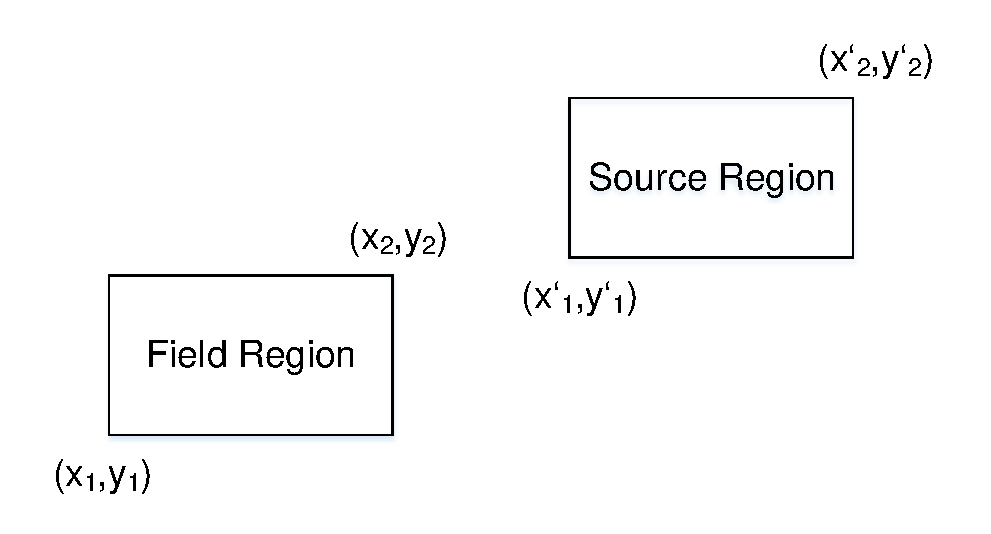
\includegraphics[width=0.8\textwidth]{__pics/regions}
	\caption{The temperature in the field region is derived from the power in the source region cf. \cite{Sapatnekar2005}}
	\label{pic:regions}	
\end{center}
\end{figure} 
\end{center}

\begin{equation}
\label{eq:hde}
\rho c_p \frac{\partial T(x,y,z,t)}{\partial t} =
\nabla \cdot [k(x,y,z,T) \nabla T(x,y,z,t)] +g(x,y,z,t)
\end{equation}

\begin{center}
	\begin{figure}[h]
		\begin{center}
			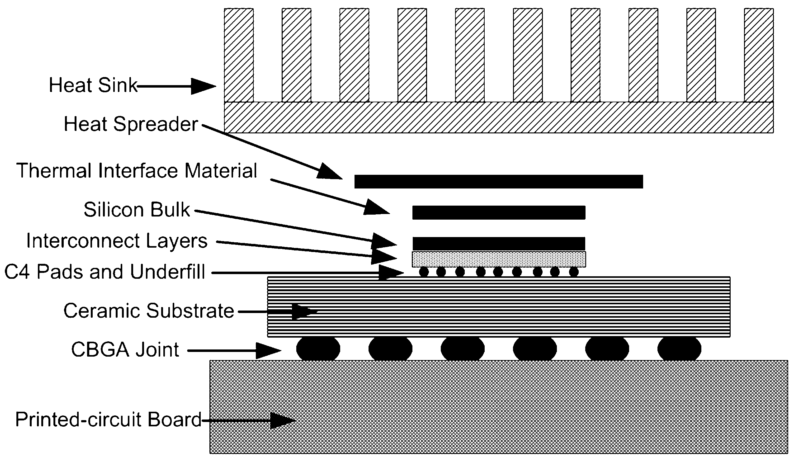
\includegraphics[width=0.8\textwidth]{__pics/packaging}
			\caption{Stacked layers in a typical \ac{CBGA} package \cite{Huang2006}}
			\label{pic:packaging}	
		\end{center}
	\end{figure} 
\end{center}

\subsection{HotSpot}
\cite{Huang2006}

\subsubsection{RC-\,Networks}

\begin{center}
	\begin{figure}[h]
		\begin{center}
			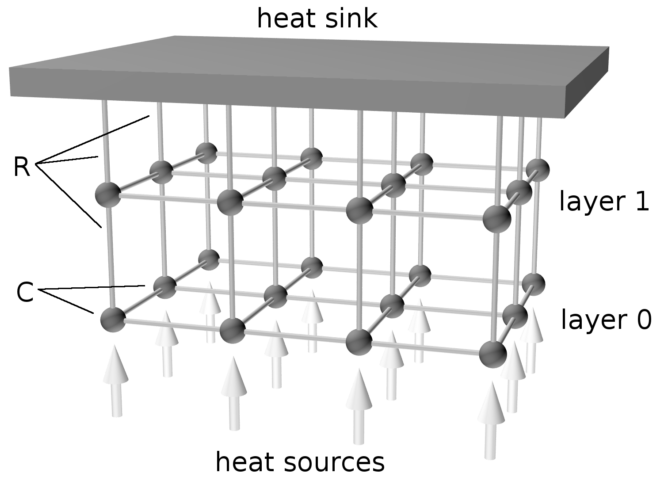
\includegraphics[width=0.7\textwidth]{__pics/rcn}
			\caption{RC-Network with two layers \cite{Happe}}
			\label{pic:rcn2}	
		\end{center}
	\end{figure} 
\end{center}


\section{Extension to On-Line Evolution of Heat Models}

\begin{itemize}
	\item RCN
	\item heat up
	\item cool down
	\item measure temperature
	\item learn parameters
	\item evaluate
\end{itemize}

\section{Temperature Measurement Methods}

\subsection{Built-In Temperature Sensor}
\label{sec:diode}
The most common way to measure temperatures on a \ac{VLSI} chip is to implement a temperature sensor in \ac{CMOS}. As stated in \cite{Bakker1996} the most effective way to achieve this goal is by using vertical bipolar transistors. This approach exploits the fact that the base-emitter voltage $V_{be}$ of a bipolar transistor decreases approximately by $2\,mV\symbol{23}^{\circ}C$ and hence almost linearly with the temperature. 
Furthermore, the difference between two measured base-emitter voltages $\delta V_{be}$ is almost linearly proportional to the absolute temperature $T_{abs}$ (ptat) and can be expressed as depicted in Equation~\ref{eq:PTAT}.

\begin{equation}
\label{eq:PTAT}
V_{ptat}(T_{abs}) = \frac{kT}{q}\cdot ln(p)
\end{equation}

The parameters for Equation~\ref{eq:PTAT} are the following:

\begin{itemize}
	\item Boltzman's constant, $k = 1.38 \times 10^{-23}$
	\item Temperature in Kelvin, $T [\symbol{23}^{\circ}\,K]$
	\item Charge on an electron in coulomb, $q = 1.6 \times 10^{-19}\,C$
	\item Emission current density ratio $p$
\end{itemize}

This temperature sensor achieves an accuracy of $\pm1\symbol{23}^{\circ}C$, by calibrating $V_{be}$ at room temperature \cite{Bakker1996}.

Also in modern \acp{FPGA} there is a trend of providing a pre-calibrated thermal diode, which are also provided at \ac{CMOS} level. These devices can for example be found at the Virtex-5 \ac{FPGA} by Xilinx, where the proportionality between the voltage and die temperature is as well exploited. Xilinx specifies this correlation with Equation~\ref{eq:XIL_PTAT} \cite{Xilinx2011a}.

\begin{equation}
\label{eq:XIL_PTAT}
V_{ptat}(T_{abs}) = 10 \cdot \frac{kT_{abs}}{q}\cdot ln(10)
\end{equation}

Note that the emission current density ratio is here set to $p = 10$. Hence, the temperature coefficient of $V_{ptat}$ is $-2\,mV/\symbol{23}^{\circ}C$.

Since the thermal diode is pre-calibrated, the temperature can be derived as depicted in Equation~\ref{eq:tempcalc}. To allow the further calculation it is mandatory to convert $V_{ptat}$, given as analog signal, into a digital number. The thermal diode on a Virtex-5 \ac{FPGA} digitizes $V_{abs}$ with the help of the built-in \ac{ADC} and produces the 10\,bit output \ac{ADC} code $V_ADC$. The resulting maximum-measurement error of this on-chip temperature sensor is specified with $\symbol{23}^{\circ}C$ \cite{Xilinx2011a}.

\begin{equation}
\label{eq:tempcalc}
	T[\symbol{23}^{\circ}C] = \frac{V_{ADC}\times 503.957}{1024} - 273.15
\end{equation}

\subsection{Infrared Cameras}
\label{sec:IRC}
Besides the above-named on-chip solutions of measuring the internal temperature, there is also the possibility to use \ac{IR} cameras. 

For instance, \cite{Ebi} measured a spatial thermal gradient of 2\symbol{23}$^{\circ}C$ over 10\,mm on a Xilinx Virtex II \ac{FPGA} using an \ac{IR} camera.
Furthermore \cite{Agne2013} used \ac{IR} cameras to illustrate temperature gradients of $15\symbol{23}^{\circ}C$, as depicted in Figure~\ref{pic:heater_infrared}. The four \ac{IR} camera pictures were taken in three second intervals. In each interval, temperature was generated in one of the chip's four corners. Inside the heated are the temperatures rose up to $95\symbol{23}^{\circ}C$ (depicted as black area), whereas the rest of the chip featured a temperature of $80\symbol{23}^{\circ}C$.

Using an \ac{IR} camera has the advantage of a high resolution. As stated in \cite{Nowroz2011}, \ac{IR} cameras can achieve a spatial resolution of up to $30\mu m$ with a $0.5\times$ microscopy kit. Furthermore, if the camera is set up properly, i.\,e. a direct view on the silicon and knowledge of the emission values, this approach provides accurate temperature information.
However, shortcomings of th \ac{IR} camera approach are that one always needs direct view on the chip's silicon layer \cite{Lopez-Buedo2004}. I.e. no heat sink, package or other material, where the emission values cannot be determined.
Besides the high price for these devices, \ac{IR} cameras cannot be employed in actual working conditions, because of their size \cite{Nowroz2011}.


\begin{figure}[h]
		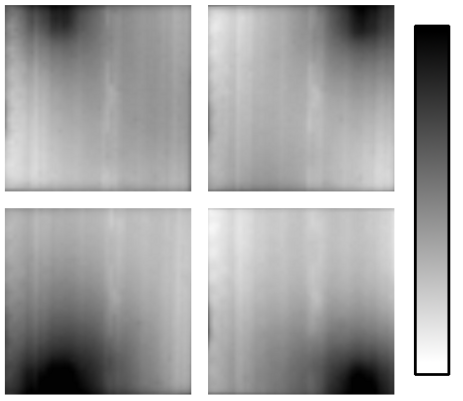
\includegraphics[width=\textwidth]{__pics/infra_heater}
		\caption{Four \ac{IR} images of the \ac{FPGA} with temperatures from 80\symbol{23}$^{\circ}C$ (white) to 95\symbol{23}$^{\circ}C$ (black) cf. \cite{Agne2013}}
		\label{pic:heater_infrared}	
	\end{figure} 

\subsection{Ring Oscillators}

Nowadays, a widely spread technique to measure the internal on-chip temperatures of \ac{FPGA}-based systems are based on \acp{RO}. These devices are composed of an odd number of inverters, which are connected in a chain. The endmost inverter's output is fed back to the first inverter. Figure~\ref{pic:simple_ro} depicts such a basic \ac{RO}. This leads to a device without a stable condition, causing each inverter's output to oscillate, i.\,e. the output $Q$ toggles between $0$ and $1$ and maximum speed with frequency $f_{osc}$. A longer inverter chain leads to a lower frequency and in addition to less power consumption \cite{Velusamy2005}.
It is because of the fact that the \ac{RO}'s frequency $f_{osc}$ is inversely proportinal to the on-chip temperature \cite{Lopez-Buedo2002}, that \acp{RO} can be used to measure the temperature on any location on the \ac{FPGA}. The output frequency $f_{osc}$ is dependant on the curcuit's delay. Furthermore, it is also known that \acp{RO} can be used in order to measure delay, leakage and dynamic power \cite{Zick2010, Zick2012}. 

\begin{figure}[h]
		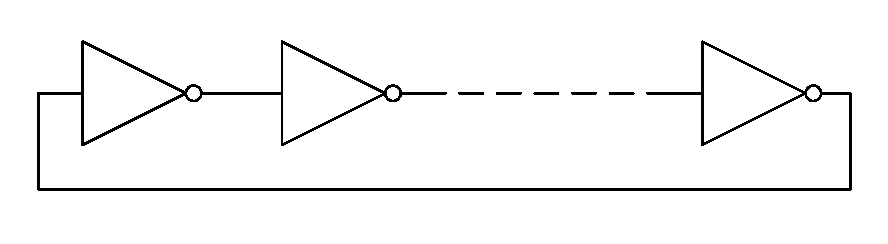
\includegraphics[width=\textwidth]{__pics/RO.pdf}
		\caption{A basic Ring Oscillator, consisting of an odd number of inverters}
		\label{pic:simple_ro}	
	\end{figure} 

\subsubsection{Methodology}

Measuring the internal on-chip temperature necessarily requires knowledge about the frequency $f_{osc}$ of the \ac{RO}. In order to estimate the frequency, several approaches \cite{Sayed2011, Lopez-Buedo2002, Velusamy2005, Happe} make use of \acp{RO} combined with a capture counter. The counter, as depicted in Figure~\ref{pic:Temp_Sensor}, is clocked with a system \ac{CLK} and by the oscillating output $Q$ of the \ac{RO}. $Q'$ toggles at the speed of $Q$ and is sampled by \ac{CLK}. Put simply, the capture counter samples the number $S$ of oscillations at the signal $Q'$ with the frequency $clk$. Afterwards the sampled number of oscillations can be derived to $f_{osc}$. 

\begin{figure}[h]
		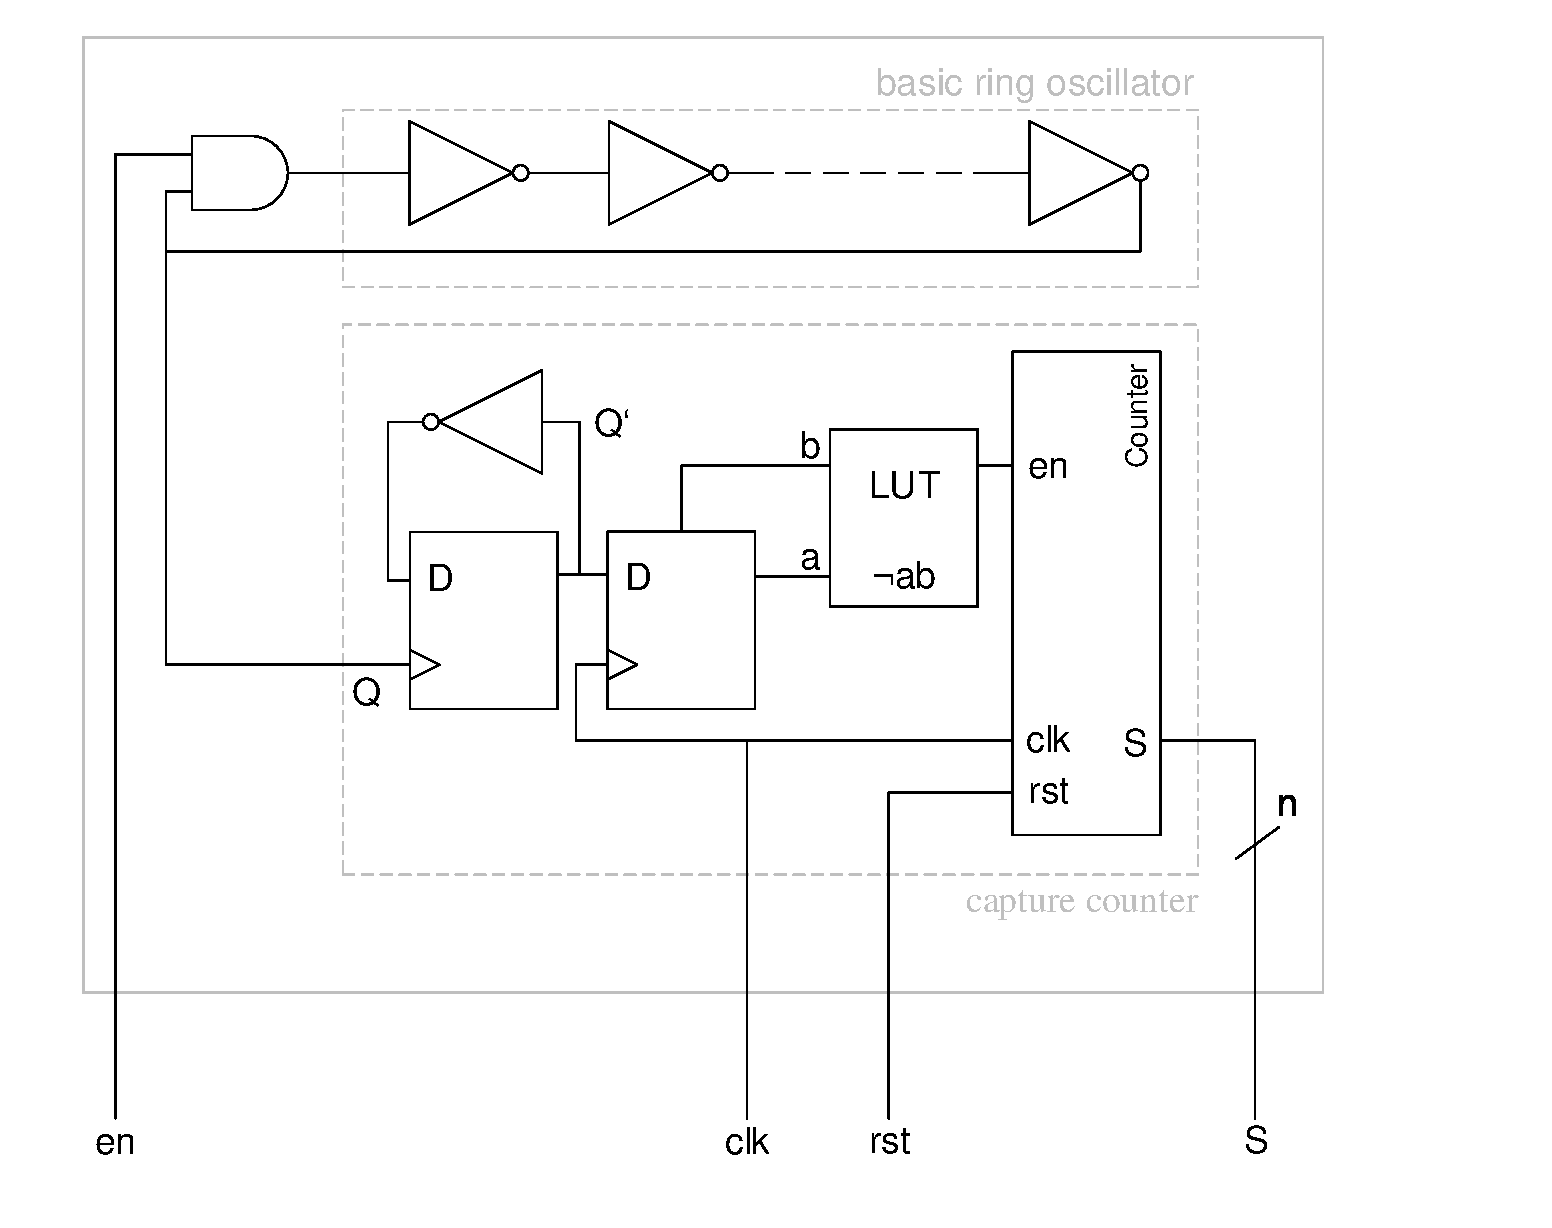
\includegraphics[width=1.15\textwidth]{__pics/Temp_Sensor.pdf}
		\caption{Simplified schematic of a temperature sensor with capture counter cf. \cite{Ruthing2012}}
		\label{pic:Temp_Sensor}	
	\end{figure} 
	
However, there are also differences in implementing the \ac{RO}-based temperature sensor. These variable parameters are: number of inverters, system routing, length of measurement period $t_m$ and the possible use of latches between the inverters. 
The use of latches was proposed in order to minimize the impact of routing \cite{Zick2012}. For \acp{FPGA} designs, it is advisable to use latches instead of the additional wiring between the inverters. 

The benefits of designing on an \ac{FPGA} are the reconfigurability. This possible due to the \acp{CLB} of which the \ac{FPGA} is composed. The \ac{CLB} however comprises slices, which contain \acp{LUT} and \acp{FF}. 
Hence, by using \acp{LUT} for the \ac{RO}'s inverters, the \acp{FF} can be used as latches without significant additional wiring.

In contrast to previous approaches, which used seven \cite{Happe} or eleven inverters \cite{Lopez-Buedo2002, Velusamy2005} and no latches, a high-performance \ac{RO}-based temperature sensor comprises 23 inverters and 24 latches \cite{Ruthing2012}. The quality of the \ac{RO} is derived by the sensor's resolution and noise/deviation.
In addition to the utilization, the optimal measurement period $t_m$ should not exceed the maximum length of $2^{16}$ clock cycles, which is $655\,\mu s$, when the counter samples with 100\,MHz. For longer measurement periods, there is a risk of self-heating, since \acp{RO} may lead to considerable temperature gradients \cite{Agne2013}.

As previously pointed out, the optimal measurement with the proposed temperature sensor includes the following steps \cite{Ruthing2012}:

\begin{itemize}
	\item Enable \ac{RO} with 23 inverters and 24 latches
  \item Wait $2^{12}$ -- $2^{16}$ clock cycles so that the \ac{RO} can gain a constant frequency
  \item Sample $Q'$ for $t_m$ clock cycles
  \item Disable the \ac{RO}
  \item Read out the counter value $S$.
\end{itemize}

\subsubsection{Calibration Methods}

Given the sensor count $S$ of \ac{RO}-based temperature sensors, it is not possible to predict a function that maps $S$ to a temperature $T$. Instead, the sensors need to be calibrated with an pre-calibrated device, such as the built-in thermal diode, a temperature-controlled oven or an \ac{IR} camera. 
While the device is heated up and cooled down afterwards, $S$ is counted and the temperature is read in regular time intervals. For each sensor placed on the chip the linear mapping function is then determined by partial regression \cite{Lopez-Buedo2002, Ruthing2012}. 

The following approaches request for a temporal temperature gradients equally distributed on the chip. Section~\ref{sec:tempgen} will give an overview of most common and useful methods for heating up the sensors, e.g. the \ac{RO}-based temperature sensors.

As proposed in \cite{Lopez-Buedo2002} the sensors were calibrated by an iron-constantan (Fe-CuNi) thermocouple which is placed in the centre of the package exactly measure the on-chip temperature $T$.

Section~\ref{sec:IRC} already illustrated that \ac{IR} cameras are able to exactly measure the on-chip temperature $T$ \cite{Nowroz2011}, provided that the camera is pointing directly on the silicon and the emission value is known. Additionally of course, they can be used for calibrating the \ac{RO}-based temperature sensors with high accuracy. 

Also, temperature-controlled ovens might be used for calibrating the sensors. Because by setting and thereby knowing the surround temperature of the die, $T$ and $S$ can also be captured.

Another way to calibrate the sensors is to make use of the built-in thermal diode, which was presented in Section~\ref{sec:diode}. While heating up the chip, the sensor data $S$ and the diode temperature $T_{diode}$ are captured. Note that this diode has $\pm 4�C$ inaccuracy and is assumed to be in the centre of the \ac{FPGA} \cite{Agne2013}.

\subsection{Discussion on Accuracy and Calibration}

The above-named approaches all fit well in the application of measuring temperatures and - if the devices are pre-calibrated - calibration of other sensors. However, each has benefits and shortcomings, which are listed in Table~\ref{tbl:proconmeasurement}. The thermal diode, which is built-in in many nowadays \acp{FPGA} benefits from being easily accessible via the system monitor. Using this temperature sensor requires no additional implementation or calibration. On the other hand the specified accuracy of $\pm 4\symbol{23}^{\circ}C$ may be to much. Furthermore, this accuracy can possibly not be met in real life. As depicted in \cite{Sayed2011}, the diode has measured incorrect temperatures compared to an external thermometer. On a Xilinx Virtex-5 \ac{FPGA} the difference between both devices amounts to $20.3\symbol{23}^{\circ}C$. Until now, it has not been resolved why this differences occurs.
Another disadvantage of using the thermal diode is that it is not clear where on the \ac{FPGA} it is placed, though it is assumed to be in the centre of the \ac{FPGA} \cite{Agne2013}. Hence the diode is not able to detect on-chip hot spots or the specific temperature of a certain instantiated circuit on the \ac{FPGA}.

A much more accurate approach is the use of \ac{IR} cameras. It is able to measure the on-chip temperatures with a high resolution, i.\,e. everywhere on the \ac{FPGA}. This again leads to the possibility of detecting hot spots.
On the other hand, \ac{IR} cameras are not only very expensive but very bulky, which hinders the in-field application. Beyond that, you need to have direct vision onto the silicon, which requires unpacking of the die.

The most effective way to measure temperatures on reconfigurable devices is using \ac{RO}-based temperature sensors. It has nearly the advantages compared to \ac{IR} cameras, and is beyond that easy to implement in reconfigurable computing devices. However, these sensor network needs to be calibrated. As this work aims to reconfigurable devices, i.\,e. \acp{FPGA}, the only handy and imaginable approach is the thermal diode, which could be a disadvantage in occurrence of incorrect measurements.


\begin{center}
\begin{table}

\begin{center}
\begin{tabular}{|p{3.16cm}|p{3.16cm}|p{3.16cm}|}
	
	\hline  \textbf{Measurement Technique} & \textbf{Pro} &  \textbf{Contra} \label{tab:proconmeasurement}\\ 
	\hline \hline  \textbf{Thermal diode} & Built-in and pre-calibrated & Inaccuracy and no hot spot detection \\ 
	\hline  \textbf{\ac{IR} camera} & Very accurate, high resolution and hot spot detection & Very expensive, no usage in field, requires view on silicon and knowledge about emission values \\ 
	\hline  \textbf{\ac{RO}-based sensor} & High resolution and hot spot detection & Calibration \\ 
	\hline
\end{tabular} 
\caption{Advantages and Disadvantages of several temperature measurement techniques}
\label{tbl:proconmeasurement}
\end{center}
\end{table}
	
\end{center}

\section{Temperature Generation Methods}
\label{sec:tempgen}

As said earlier most sensors, e.\,g. \ac{RO}-based, have to be calibrated before use. In order to do so accurately, the \ac{IC} needs to be heated up to learn about the sensor output in combination with a pre-calibrated sensor temperature output.
But besides that, it might be interesting to heat up devices for the sake of evaluating the functionality. This may include fault tolerance like timing or soft and hard errors under occurrence of heat, especially for scientific use.

Several approaches are using a temperature-controlled oven in order to heat up the chip \cite{Velusamy2005, Lopez-Buedo2002}. This way, the \ac{IC} is heated up and simultaneously the \acp{RO} are calibrated. In the first instance, these approaches use heat generation for calibration. But as a matter of principle, temperature controlled ovens can be used to heat up \acp{IC} uniformly distributed on the die.
Practically, on the other hand, it might also be interesting to create local hot spots and generate spatial gradients on the chip in order to learn about the chip's thermal properties. Temperature controlled ovens do not support this kind of researching, not least because of the needed bulky external device.
A much handier way to calibrate sensors might be the laser trimming \cite{Bakker1996}, which is out of place in the field of reconfigurable computing, for instance for designing on \acp{FPGA}.

A better way, which also perfectly matches the advantages of reconfigurable computing is the use of dedicated heat generating circuits, specified in Verilog or \ac{VHDL}, following the approach of self-heating. By instantiating the low level components of a \ac{FPGA}, several approaches achieved temperature increases and local hot spots on the die. These components are mostly placed in the \ac{FPGA}'s \ac{CLB} and comprise

\begin{figure}[h]
	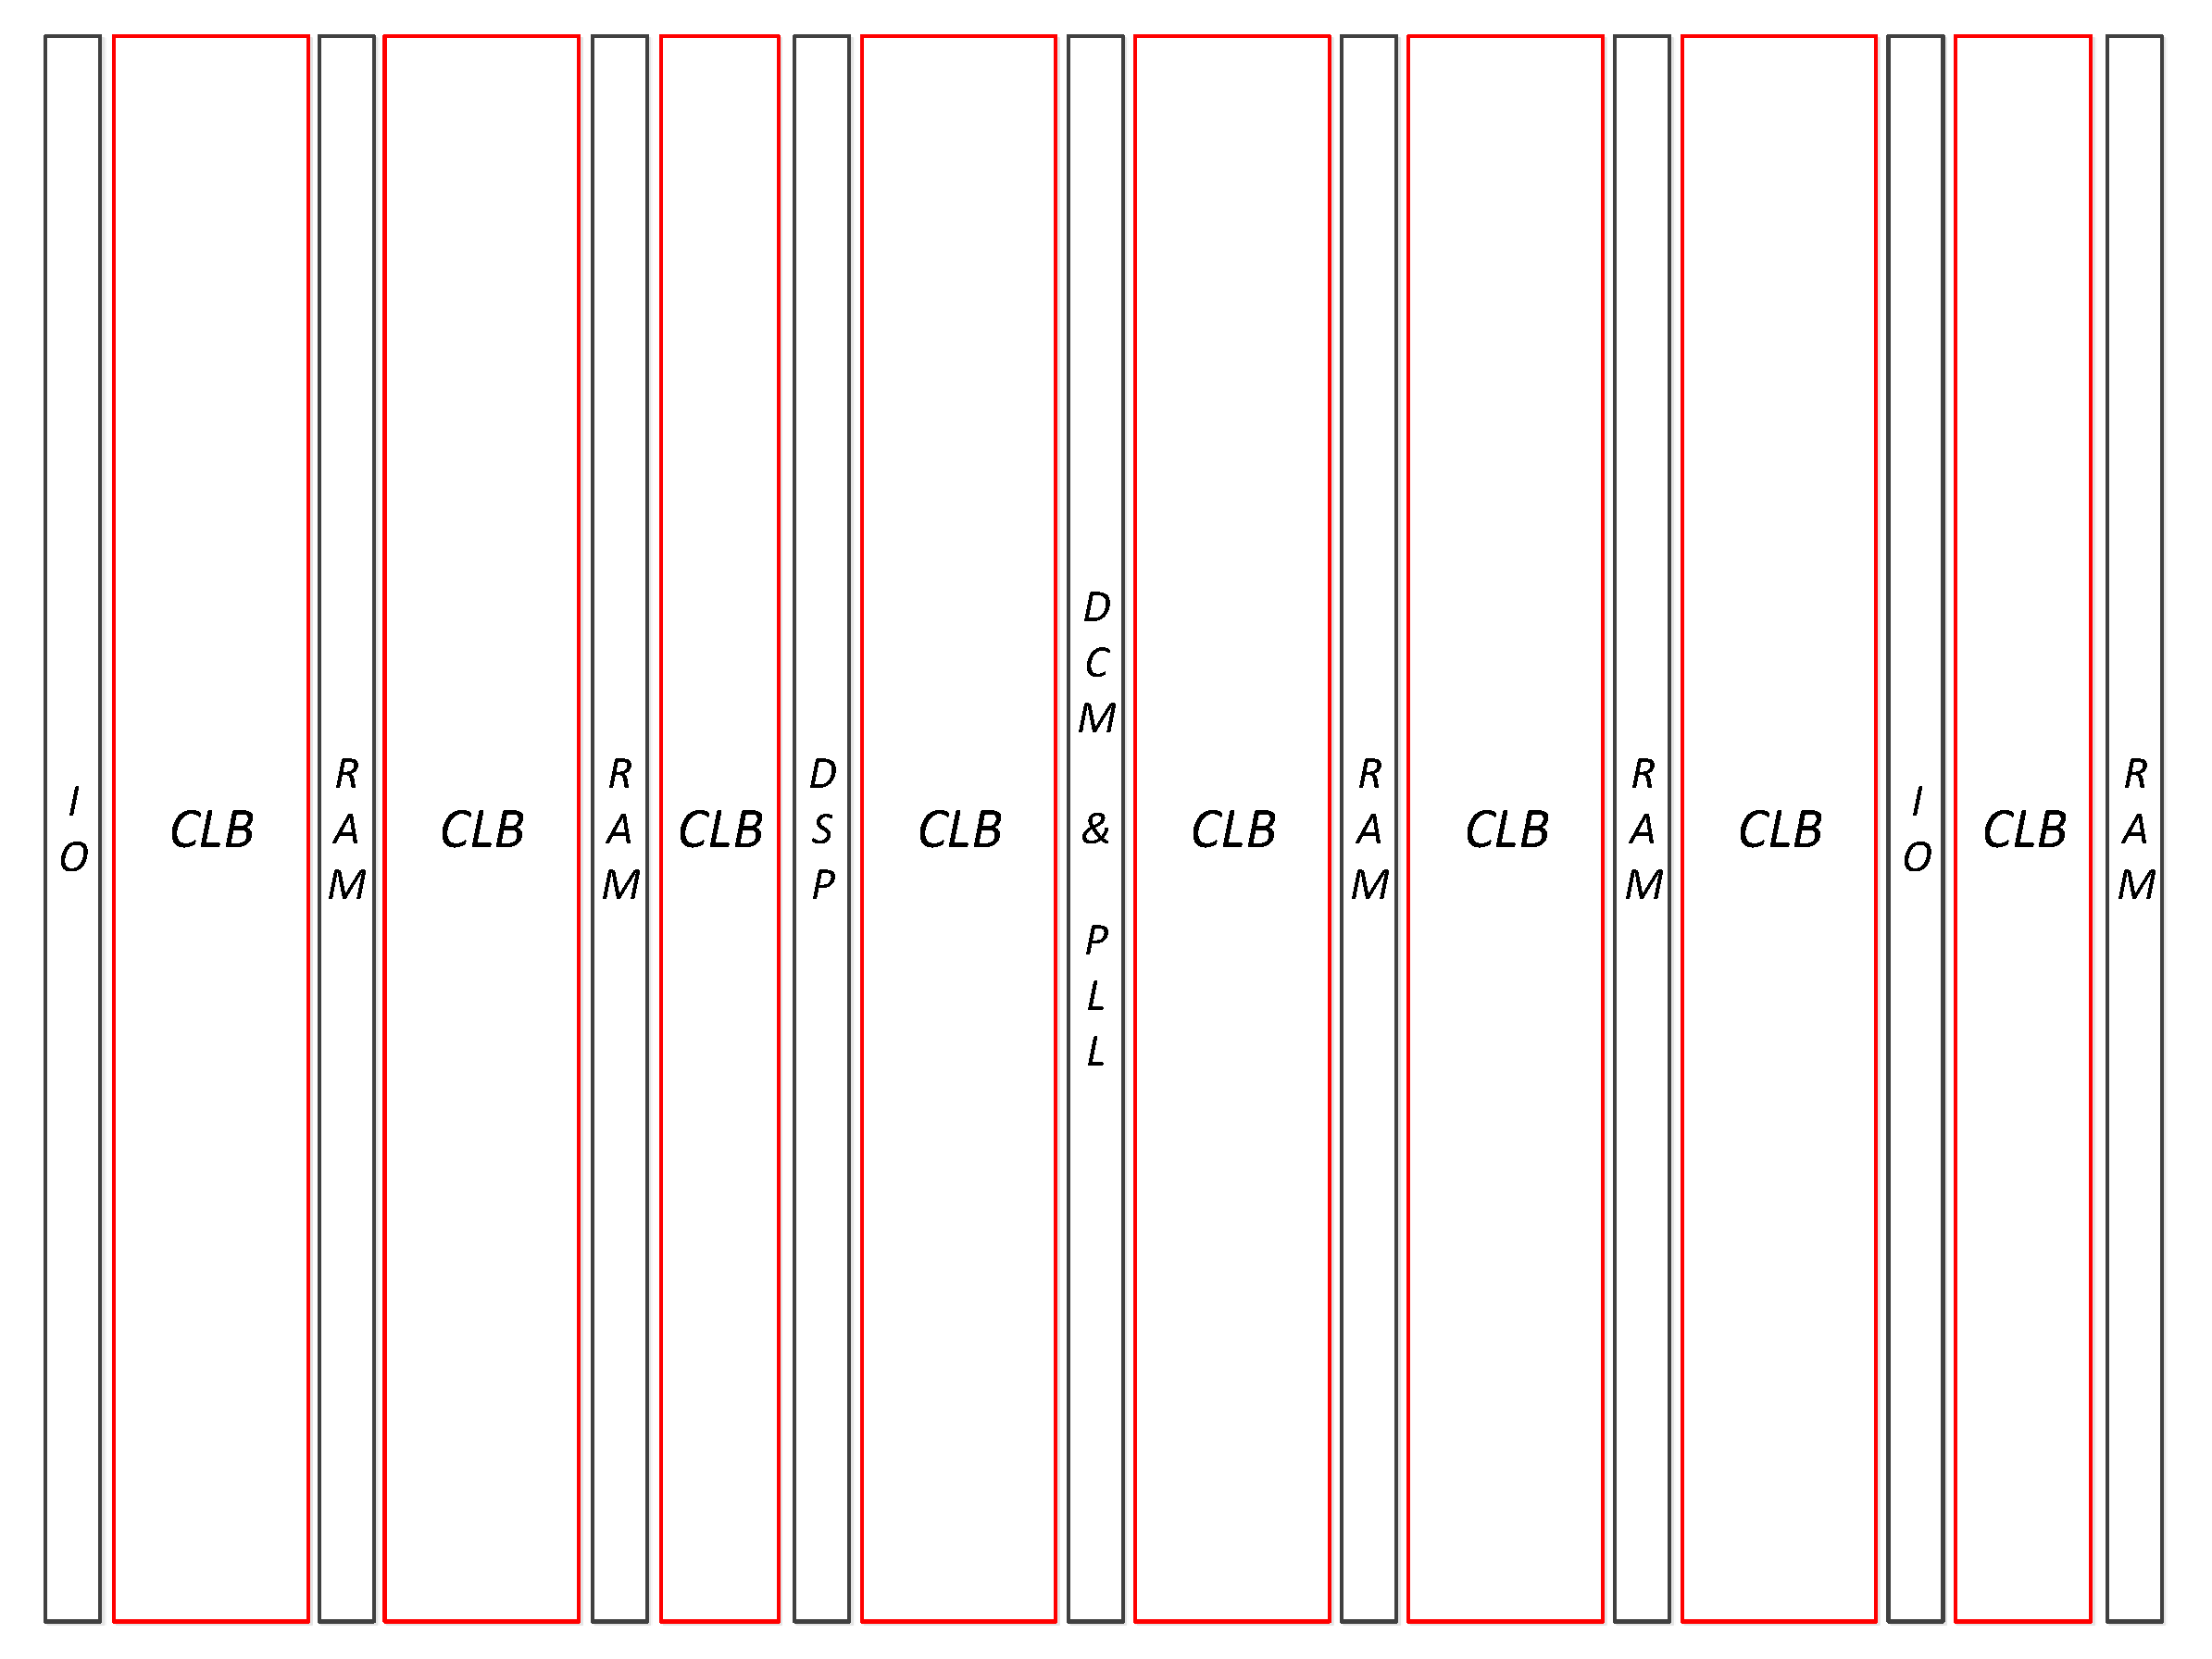
\includegraphics[width=\textwidth]{__pics/v5.pdf}
	\caption{A simplified overview of a Virtex-5 \ac{FPGA}}
	\label{pic:v5}	
\end{figure}

\begin{itemize}
	\item \acp{LUT}\\
			Arranged in the \ac{CLB}'s slices. \acp{LUT} can implement any \textit{n}-input logic function. The highest amount of input signals \textit{n} is nowadays 6. Logical functions with a higher amount in input signals can be achieved by combining several \acp{LUT}
	\item \acp{FF}\\
			Also stored in slices next to \acp{LUT}. \acp{FF} can be initialized with a start value.
	\item \acp{DSP}\\
			\ac{DSP} blocks are compact and high-speed circuits and fulfil the special purpose of huge arithmetical and logical operations. Usually there is a special area between some \acp{CLB}
	\item \acp{BRAM}\\
	       Also arranged between several \ac{CLB}. \acp{BRAM} can for instance be used as \ac{FIFO}, single or dual port \ac{RAM}.
\end{itemize}

Figure~\ref{pic:v5} depicts the arrangement of these components on Virtex-5 \ac{FPGA}. Additionally \ac{IO} blocks, \ac{DCM} and \ac{PLL} are added.

It is easy to see that the most effective way to generate temperature increases and especially local hot spots or spatial temperature gradients is to use the \acp{CLB}, i.\,e. \acp{LUT} and \acp{FF}. The designer is thereby almost not restricted to an area that can be heated. 
As illustrated in \cite{Sayed2011} the used \ac{FPGA} increased its temperature up to 37$\symbol{23}^{\circ}C$ by utilizing $80\%$ of the \acp{CLB}. More precisely, the \acp{LUT} and \acp{FF} were arranged in a pipeline as depicted in Figure~\ref{pic:lutffpipe}, clocked at $100\,MHz$. The output of each \ac{LUT} was wired with the input of another \ac{FF}, whose output was on the contrary was wired to another \ac{LUT} and so on.

\begin{figure}[h]
	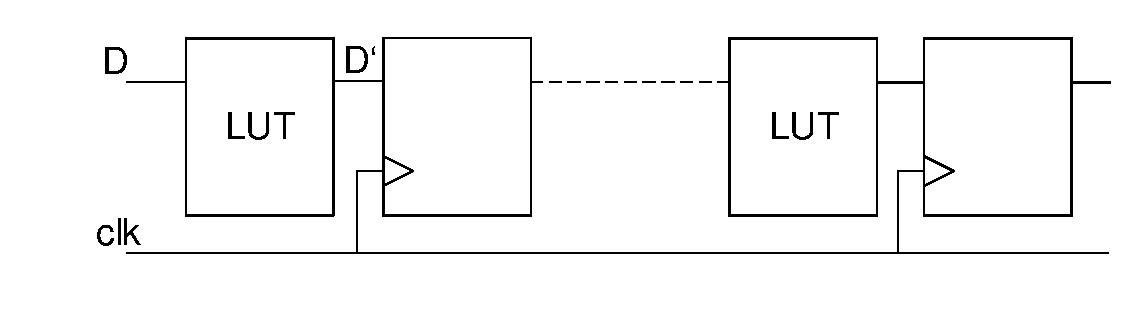
\includegraphics[width=\textwidth]{__pics/LUTFFpipe.pdf}
	\caption{ Pipeline consisting of \acp{LUT} and \acp{FF}}
	\label{pic:lutffpipe}	
\end{figure}

\begin{figure}[h]
	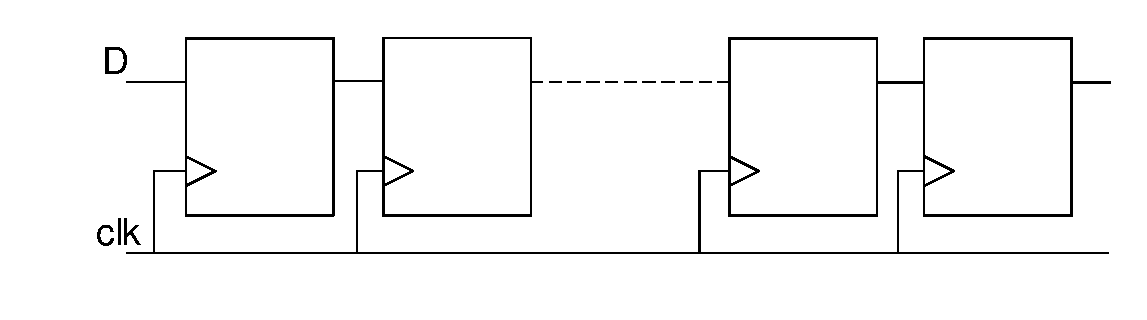
\includegraphics[width=\textwidth]{__pics/FFpipe.pdf}
	\caption{Pipeline consisting of \acp{FF} }
	\label{pic:ffpipe}	
\end{figure}

Local hotspots were for instance created by using a \ac{FF} pipeline as illustrated in Figure~\ref{pic:ffpipe}. As \cite{Happe} depicted, it is possible to create a spatial gradient of $6.5\symbol{23}^{\circ}C$ by utilizing 10.000 \acp{FF} on the \ac{FPGA}, which were clocked at $100\%$.

As a systematic study of possible heat generating circuits yielded, there are even more temperature increases and spatial gradients possible \cite{Agne2013}. A average overall temperature rise of $81.2\symbol{23}^{\circ}C$ was achieved by implementing 1.000 single-level oscillators on the \ac{FPGA}. As Figure~\ref{pic:lutosc} depicts, this oscillators were realized with \acp{LUT}, which fed back the outputs to the input \textit{I0}. The logical function that was stored in this \ac{LUT} is a simple \ac{XOR}, which function as an inverter, when the enabling signal is activated. This slim and effective heat generating circuit also achieved a spatial temperature gradient of up to $10\symbol{23}^{\circ}C$.

\begin{center}
\begin{figure}[h]
\begin{center}
	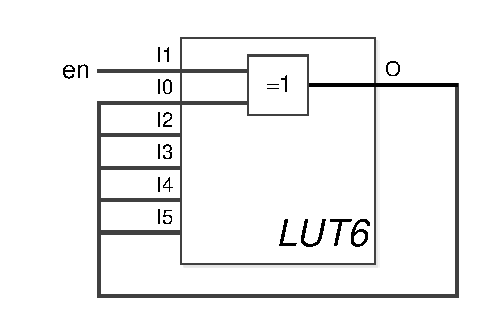
\includegraphics[width=0.70\textwidth]{__pics/lutoscillator.pdf}
	\caption{\ac{FPGA}-Implementation of a 1-level \ac{RO}}
	\label{pic:lutosc}	
\end{center}
\end{figure} 	
\end{center}
\cleardoublepage


\chapter{Online Evolution of Heat Models}
\label{ch:onlineevo}


\section{Temperature Model Definition}

The temperature model is basically as defined in Section~\ref{ch:hotspot} and Section~\ref{ch:ext}.

\begin{itemize}
	\item RCN
	\item heat up
	\item cool down
	\item measure temperature
	\item learn parameters
	\item evaluate
\end{itemize}

\begin{equation}
\label{eq:mse}
mse(P)=\frac{1}{|N||M|} \cdot \sum_{i\in M} \sum_{j\in N} (T_s(P,t_i,j)-T_m(t_i,j))^2
\end{equation}

\section{Learning and Optimizing Algorithms}
\subsection{Simulated Annealing}

\subsection{Evolutionary Algorithms}
\subsection{Metropolis Algorithms}

\subsection{Gradient Descent Algorithms}

\subsection{Particle Swarm Optimizations}

\subsection{Hill Climbing}
\subsection{Evolutionary Algorithms}
\cleardoublepage

 
\chapter{Experiments and Evaluation}
\label{ch:experiments}

\begin{itemize}
\item{Experiments on RC-network}
\item{Results for several Learning Algorithms}
\item{Discussion of Convergence}
\item{Discussion of Accuracy}
\item{Discussion of On-Line Suitability}
\item{Discussion of Embedded Implementation}
\end{itemize}

\cleardoublepage

%!TEX root = /Users/nphs/Dropbox/0-Bachelor/2012-BA-Cioran/02-Arbeit/BA-Cioran.tex
\chapter{Conclusion}
\label{ch:conclusion}

In this thesis I have presented crazy shit!
\cleardoublepage

	%%!TEX root = /Users/nphs/Dropbox/0-Bachelor/2012-BA-Cioran/02-Arbeit/BA-Cioran.tex
\chapter{Problemdefinition}
\label{ch:problem}

There are several different ways to develop dedicated heat- generating circuits on a \ac{FPGA}. The \ac{FPGA} consists of three main parts: Slices, \acp{BRAM} and \acp{DSP}. These components get wired dynamically, depending on the desired functionality. The functionality is described in Hardware Description Languages such as \acp{VHDL}. Slices consists of several \acp{LUT} and \acp{FF} and can be combined to any desired circuit. \acp{DSP} are hard-\,coded circuits for special uses, e.\,g. calculations. By the reason that e.\,g. multipliers would take a high amount of space if they were realized by \acp{LUT} and \acp{FF}, these tasks are mapped to special processors for that purpose. Because of their special purpose, they are highly space-\,saving. \acp{BRAM} are memory units. It is possible to instantiate Slices (\acp{LUT} and \acp{FF}), \acp{DSP} or \acp{BRAM} and use them specifically for heat-\,generating circuits. During the research it is eligible to identify the part that generates the most heat and research if the mixture of parts outperforms that solution. Furthermore the frequencies of these parts are varied to measure the influence of diverse clocking.
	%\cleardoublepage
	%
	%
\chapter{Technical Background}
\label{ch:technical}
\section{FPGAs}
\label{ch:fpgas}

An \ac{FPGA} is an \ac{IC} on which logical circuits can be implemented. More specifically an \ac{FPGA} is a semiconductor device that is based around a matrix of \acp{CLB} connected via programmable interconnects \cite{Xilinx}. \acp{CLB} are the logical blocks, where most of the sequential as well as combinatorial circuits will be implemented. Each of them consist of a pair of slices, which are not directly connected to each other \cite{Xilinx2012a}. Each of this slices contains \acp{LUT} and \acp{FF}. Basic logical functions such as AND, OR and so an are mapped into the \acp{LUT} by defining a table with all input constellations and their corresponding outputs. There are no hard-\,wired logical functions in a \ac{LUT}. 
The other components which are located in a \graffito{slice} slice, are \acp{FF}. \acp{FF} are 1-bit registers and can store one bit over any amount of time. 

\begin{figure}[h]
		\includegraphics[width=\textwidth]{__pics/FPGA}
		\caption{Basic design of an FPGA \cite{Website}}
		\label{pic:fpga}	
	\end{figure}

Additionally there are a few more components, which can be configured in order to achieve the desired logical circuit. Besides \acp{CLB} these components are \acp{DSP} and \acp{BRAM}. A \ac{DSP} is an \ac{ASIC}, i.\,e. a hard-wired logic whose specific functions are huge arithmetical and logical operations. By the reason that e.\,g. multipliers would take a high amount of space if they were realized by \acp{LUT} and \acp{FF}, these tasks are mapped to special processors for that purpose. Because of their special purpose, they are highly space-\,saving. A \ac{BRAM} is a simple \ac{RAM}, which is a memory unit. Figure \ref{pic:fpga} shows an exemplary structure of a \ac{FPGA}. Besides the logic blocks, it depicts the programmable interconnects and \ac{IO} blocks.


As already said above, these components are connected via a programmable interconnects, which make the \ac{FPGA} reconfigurable \cite{Dubey2009}. These programmable interconnects consist of horizontal and vertical wires and switches (antifuse or pass transistors) \cite{Www.ycce.edu}, which route the signals between the components of the \ac{FPGA}. So, via configurating the switches, the components can be wired.

\begin{figure}[h]
		\includegraphics[width=\textwidth]{__pics/HDLtoBIT}
		\caption{From HDL-file to configuration bitfile}
		\label{pic:hdltobit}	
	\end{figure} 

As a first step to configure a \ac{FPGA} with the desired hardware function, the hardware has to be described by a \ac{HDL} such as Verilog or \ac{VHDL}. Secondly the described hardware will be synthesized in order to get a logical circuit (Figure \ref{pic:hdltobit}). At this point the hardware can be easily run in a simulation, but can not be loaded on the \ac{FPGA}, because foremost the logical circuit has to be mapped to the specific \ac{FPGA} architecture. Therefore, the logical circuit has to be implemented to a configuration bitfile. This bitfile contains the configuration of every component on the chip, e.\,g. the logical function function of a \ac{LUT}, the start value of a \ac{FF} or the programmable interconnects.

\begin{figure}[h]
		\includegraphics[width=\textwidth]{__pics/virtex5}
		\caption{A simplified overview of a Virtex-\,5 FPGA}
		\label{pic:virtex5}	
	\end{figure} 


\section{Target Device}
\label{sec:target}
For this work a \textit{Xilinx Virtex-\,5} \ac{FPGA} (xc5vlx110t) was used, which has a maximum supported working temperature of 120\symbol{23}$^{\circ}$C. Furthermore the Virtex-\,5 is equipped with a diode, which enables the reading of the temperature and the supply voltage of the chip. The Circuits on the Virtex-\,5 can be implemented with a maximum frequency of 600\,MHz.

\begin{figure}[h]
		\includegraphics[width=\textwidth]{__pics/CLB}
		\caption{Composition of the CLB column in Figure \ref{pic:virtex5}}
		\label{pic:clb}	
	\end{figure} 

Figure \ref{pic:virtex5} shows a simplified overview of the chip. As you can see, the Virtex-\,5 consists of eight \ac{CLB} columns, five \ac{BRAM} columns and one \ac{DSP} column. There are also areas for the \ac{DCM} and the \ac{PLL}, which are used for the clock generator. \ac{IO} columns are needed to interact with the hardware on the \ac{FPGA}. The amount of \acp{BRAM} is 148, with a memory size of 36\,Kb each. Additionally they can also be used as two \acp{BRAM} with 18\,Kb. The maximum memory in \acp{BRAM} is 5328\,Kb. The amount of available \acp{DSP} is 64 \cite{Description2009}. 


\begin{center}

\begin{figure}[h]
\begin{center}
		\includegraphics[width=0.6\textwidth]{__pics/slice}
		\caption{Composition of slice}
		\label{pic:slice}	
		\end{center}
	\end{figure} 
\end{center}

The main parts of the chip are the \acp{CLB}. There are two types of \acp{CLB}: first the \textit{CLBLM}, which consists of one \textit{SliceM} and one \textit{SliceL} and secondly the \textit{CLBLL}, which consists of two \textit{SliceLs}. Just as the \textit{SliceL}, the \textit{SliceM} contains four \acp{LUT} and four \acp{FF}, as Figure \ref{pic:slice} depicts. The only difference is, that a \textit{SliceM} can be configured to operate as a 32-bit shift register or as a 64-bit distributed RAM \cite{Description2009}. Every row in the \ac{CLB} matrix is in the same sequence as shown in Figure \ref{pic:clb}.

\section{Xilinx Primitives}
\label{sec:primitives}

This chapter provides an overview of what Xilinx primitives are and how they are used. The chapters are ordered by the primitives, which are used in this thesis. 

Xilinx primitives are hardware structures, which can be instantiated like any other circuit, even though they are not existent in a Hardware Description Language like \ac{VHDL}. In fact, they are already implemented and available as netlists. These netlists can now be easily integrated and instantiated in the \ac{VHDL} code. 

The special feature of the primitives is that these circuits are native to the targeted \ac{FPGA} \cite{Xilinx2010c}. For example, you are able to instantiate \acp{FF}, \acp{DSP} and many more components, which will be directly mapped to the corresponding hardware devices on the \ac{FPGA}. 

This chapter should give you a closer look on the five primitives that are used to implement the following circuits. 

\begin{itemize}
	\item \acp{LUT}
	\item \acp{FF}
	\item \acp{SRL}
	\item \acp{DSP}
	\item \acp{BRAM}
\end{itemize}

\subsection{Lookup Tables}

\begin{figure}[h]
	\center
		\includegraphics[width=0.7\textwidth]{__pics/LUT6.pdf}
		\caption{Structure of a LUT6, c.\,f. \cite{Xilinx2010c}}
		\label{pic:lut6}	
	\end{figure} 

\acp{LUT} are the basic logic building blocks in the hardware, since they can implement any \textit{n}-\,input logic function, where \textit{n} is the amount of input signals \cite{Xilinx2010c}. Therefore a matrix with all possible inputs and the consequential output is stored in the \ac{LUT}.

The \acp{LUT} on the Virtex-\,5 \ac{FPGA} feature up to six input signals and either one or two output signals (\textit{O}). I.\,e. \ac{LUT6} \graffito{LUT6} can implement any logic function with six input signals (\textit{I0} to \textit{I5}). The basic structure of a \ac{LUT6} is depicted in Figure \ref{pic:lut6}. As you can see the \ac{LUT6} is arranged with the help of two \ac{LUT5}\graffito{LUT5}. Therefore it is possible to use two \ac{LUT} primitives on the Virtex-5 \ac{FPGA}: with six or only five input signals.

There is also the possibility to use a second output signal of the \ac{LUT6}, which would simply be the output signal of the lower \ac{LUT5}.

Beyond that, it is also possible to use a \ac{LUT} as an asynchronous 64\,bit ROM, which is addressed with the 6 input signals \cite{Xilinx2010c}.
	
	
\subsection{Flip-Flops}

	\begin{figure}[h]
		\center
		\includegraphics[width=0.55\textwidth]{__pics/FDCPE.pdf}
		\caption{D Flip-\,Flop with Clock Enable Asynchronous Preset and Clear, c.\,f. \cite{Xilinx2010c}}
		\label{pic:fdcpe}	
	\end{figure}

An \ac{FF} is a bistable circuit and can be in two solid states, in order to store a single bit over any amount of time. In addition, \acp{FF} are clock-\,controlled, which means the \ac{FF} is only able to change its state, when a rising edge of the clock arrives. 

Figure \ref{pic:fdcpe} depicts a D-\,type \ac{FF} with one output signal (\textit{Q}), which can be used on the Virtex-\,5. In addition to the input signal (\textit{D}) and the \ac{C}, this \ac{FF} has also an \ac{PRE}, an \ac{CLR} and a \ac{CE}. The \ac{PRE}-\,signal is to preset the value of the \ac{FF} and is independent of the \ac{CLK}. The \ac{CLR}-\,signal is as well independent of the \ac{CLK} and can asynchronously clear the value of the \ac{FF}. \ac{CE} simply enables or disables the \ac{FF} depending on whether it is 0 or 1.  This constellation gave this primitive the name \graffito{FDCPE} \ac{FDCPE}.



\subsection{Shift Register Lookup Tables}

	\begin{figure}[h]
		\center
		\includegraphics[width=0.55\textwidth]{__pics/SRL16E.pdf}
		\caption{16\,bit Shift Register Lookup Table with Clock Enable, c.\,f. \cite{Xilinx2010c}}
		\label{pic:srl16e}	
	\end{figure}

The \ac{SRL} is a \ac{LUT} which acts like a shift register. A shift register on the other hand is normally a cascade of \acp{FF} whose input is their predecessors output. I.\,e., a shift register passes a bit through all its \acp{FF}.

There is a way that a 16\,bit shift register is not mapped to 16 \acp{FF}, but only to one \ac{SRL}. This primitive is called \ac{SRL16}. Figure \ref{pic:srl16e} depicts the basic structure of a \ac{SRL16E}\graffito{SRL16E}, which is the same as a \ac{SRL16}, except the enabling input signal. The \textit{D}, \ac{CE}, \ac{C} and \textit{Q} signals are the same as used by the \ac{FDCPE}. The input signals \textit{A0} to \textit{A3} are needed for the configuration of the \ac{SRL16E}.

But \acp{SRL16} can not be mapped to every \ac{LUT}. As chapter \ref{sec:target} described, there are two types of slices (\textit{SliceL} and \textit{SliceM}). \acp{SRL16} can only be mapped to the \acp{LUT} in a \textit{SliceM}.


\subsection{Digital Signal Processors}

	\begin{figure}[h]
		\center
		\includegraphics[width=0.70\textwidth]{__pics/dsp.pdf}
		\caption{Strongly simplified structure of a DSP, c.\,f. \cite{Xilinx2010c}}
		\label{pic:dsp}	
	\end{figure} 

\acp{DSP} are compact and high-\,speed circuits and fulfill the special purpose of huge arithmetical and logical operations. Multiplications calculated with \acp{LUT} and \acp{FF} would firstly suffer from the used space on the chip and secondly from the elapsed time for the operation. Hence, huge arithmetical and logical operations are mapped to \acp{DSP}.

The Virtex-\,5 primitive \graffito{DSP48E}\ac{DSP48E}  features several arithmetical and logical operations on two's complement values. It is possible to multiply up to 25-\,bit value by an 18-\,bit value. If the multiplier is not used, the \ac{DSP48E} can also be used as a full 48-\,bit adder or subtracter. Additionally there is an alternative of using a hybrid, which contains firstly a multiplier operation and secondly an add, subtract or round operation \cite{Xilinx2012b}. 

Figure \ref{pic:dsp} depicts a strongly simplified overview of the \ac{DSP48E} structure. The input signals A and B are used for multiplication, with the limitation that only the lower 25 bits of A will by multiplied with the 18\,bit long input signal B. Subsequent to the multiplication it is possible to add or subtract the 48\,bit long input signal C. In order to use the full 48\,bit adder/subtracter, A delivers 30\,bit \ac{MSB} input and B delivers 18\,bit \ac{LSB} input to the adder. Thus, A and B get concatenated and afterwards added/subtracted to C \cite{Xilinx2010c}.

Besides the aforesaid operations the \ac{DSP48E} on the Virtex-\,5 \ac{FPGA} is also capable for accumulation, shifting, logical operations and pattern detection, which get directed by the input signals OPMODE and ALUMODE. There are a lot of more input and output signals, which will be abandoned at this point. The maximum frequency for this \ac{DSP} is 550\,MHz.

\subsection{Block RAMs}

There are several ways to use a \ac{BRAM} on a Virtex-5. These varieties are \acp{FIFO}, automatic error-\,correction \ac{RAM}, or general-purpose 36\,kb or 18\,kb \ac{RAM}/\ac{ROM} memories \cite{Xilinx2010c}. Above that, these \acp{BRAM} can be configured as single port \ac{RAM} or dual port \ac{RAM}. This work will deal with a \graffito{FIFO36}\ac{FIFO36}.

\begin{figure}[h]
		\includegraphics[width=\textwidth]{__pics/bram.pdf}
		\caption{Simplified structure of a BRAM, c.\,f. \cite{Xilinx2010c}}
		\label{pic:bram}	
	\end{figure} 
	
		
Figure \ref{pic:bram} depicts a simplified \ac{BRAM}, which can be used as a \ac{FIFO36}. Besides the \ac{RST} the \ac{FIFO} has got two enable signals, \ac{RDEN} and \ac{WREN}. The output signals are \textit{EMPTY} and \textit{FULL}, which are 1 if the \ac{BRAM} is either full or empty. Furthermore, there are two buses, which handle the data reading and writing. The widths $x$ of the \ac{DI} and the \ac{DO} can be configured to four different widths: $x = 4, 8, 16$ or $32\,bit$.
	%\cleardoublepage
	%
	%%%!TEX root = /Users/nphs/Dropbox/0-Bachelor/2012-BA-Cioran/02-Arbeit/BA-Cioran.tex
\chapter{Konzeption und Modellierung}
\label{ch:konzeption}
Dieses Kapitel gibt einen �berblick �ber die zu implementierenden Funktionen und das \ac{UI} der zu entwickelnden Applikation \emph{ginkgo mobile}. Das Ziel dabei ist eine neue Erfahrung f�r die Teilnehmer von wissenschaftlichen Konferenzen zu erm�glichen. Daf�r werden im Abschnitt \ref{sec:ginkgoFeatures} die f�r \emph{ginkgo mobile} relevanten Funktionen des \ac{CMSs} \emph{ginkgo} erkl�rt. Die wichtigsten daraus resultierenden \emph{Use Cases} und die notwendigen Komponenten zur Implementierung werden im Abschnitt \ref{sec:ginkgomobile} beschrieben. 

\section{ginkgo Features}
\label{sec:ginkgoFeatures}
Registrierte Benutzer haben ein eigenes Profil, indem Informationen �ber die eigene Person, wie Interessen und Arbeitgeber, angezeigt werden. Durch die Profile ist jeder Nutzer identifizierbar. Dadurch k�nnen Nutzer anderen Nutzern \emph{folgen},  sich private Nachrichten senden und Status Updates posten. \graffito{Activity Stream} �ber die Liste der registrierten Veranstaltungen lassen sich Informationen zu einzelnen Events anzeigen, die im \emph{veranstaltungsbezogenen Activity Stream} auf der jeweiligen Seite der Konferenz angezeigt werden. Dabei handelt es sich beispielsweise um ge�nderte Fristen, angenommene Paper und neue Reviewer. Des Weiteren lassen sich Personen anzeigen, die dem jeweiligen Event \emph{folgen} oder an der Veranstaltung \emph{teilnehmen} wollen. Durch die M�glichkeit einem Event zu \emph{folgen}, werden die Informationen des jeweiligen \emph{veranstaltungsbezogenen Activity Stream} auch in dem pers�nlichen \emph{Global Activity Stream} angezeigt. Dieser zeigt zus�tzliche Informationen zu Status Updates von dem jeweiligen Nutzer und seinen Freunden an. 

\section{ginkgo mobile}
\label{sec:ginkgomobile}
\subsection{Use Cases}
Im folgenden Abschnitt wird eine Auswahl an wichtigen \emph{Use Cases} gegeben.
\subsubsection{Informationen zu Usern und Events}
Der Nutzer soll Informationen zu jedem \emph{User} und zu jedem \emph{Event} abfragen k�nnen.
\subsubsection{Die Anzeige von Activity Streams}
Zu jedem \emph{Event} und jedem \emph{User} soll der jeweilige \emph{Activity Stream} angezeigt werden k�nnen. Dar�ber hinaus soll dem Nutzer die M�glichkeit zum verfassen von eigenen Status Updates gegeben werden. 

\subsubsection{Private Nachrichten}
Kommunikation zwischen Nutzern soll durch private Nachrichten erm�glicht werden.

\subsubsection{Landkarte}
Auf einer Landkarte sollen dem Nutzer alle umliegende \emph{Events} angezeigt werden.

\subsubsection{Friends/Follower anzeigen}
Durch die \emph{Friends} und \emph{Follower} eines \emph{Users} soll durch einen \emph{ViewPager} navigiert werden k�nnen.

\subsection{Geplante Android Komponenten und deren Verhalten}
\label{sec:ginkgomobilekomponenten}
Die neu zu erstellende \emph{LoginActivity} wird als Einstiegspunkt in \emph{ginkgo mobile} dienen. Nach Eingabe der Benutzerdaten wird bei einer erfolgreichen Authentifizierung die \emph{DashActivity} gestartet (siehe Abbildung \ref{pic:mock_globaldash}). Diese besteht aus dem DashboardFragment und einer View (siehe Abschnitt \ref{sec:androidprog}), die als Container f�r Fragments dient. Zu Beginn enth�lt der Container das \emph{ActivitystreamFragment} um den \emph{Global Activity Stream} (siehe Abschnitt \ref{sec:ginkgoFeatures}) des eingeloggten Nutzers anzuzeigen.
\begin{figure}[h]
	\includegraphics[width=\textwidth]{__pics/diagramme/dashkonzept_blockd}
	\caption{Nach einem erfolgreichen Login wird die DashActivity gestartet. Diese besteht aus dem DashboardFragment und einem Container der andere Fragments beinhaltet.}
	\label{globalDash}
\end{figure}

Durch Interaktionen des Nutzers mit dem \emph{DashboardFragment} kann die \emph{DashActivity} das zur Zeit im Container angezeigte Fragment durch ein anderes ersetzen. Die m�glichen Fragments, die der Container beinhalten kann, werden im Folgenden erkl�rt. 
\begin{itemize}
	\item \textbf{UserFragment}
	
	Das {UserFragment} kann sowohl das Profil des eingeloggten Nutzers als auch Profile anderer Personen anzeigen. Dazu geh�ren pers�nliche Informationen und der jeweilige \emph{Global Activity Stream}. Um den jeweiligen Nutzer zu folgen (siehe Abschnitt \ref{sec:ginkgoFeatures}) gen�gt ein Klick auf den \emph{Follow} Button. �ber den \emph{Message} Button kann der Person eine private Nachricht schreiben (siehe Abbildung \ref{pic:mock_profile}).
	\item \textbf{ActivitystreamFragment}
	
	Durch das \emph{ActivitystreamFragment} k�nnen sowohl \emph{Global Activity Streams} als auch \emph{eventbezogene Activity Streams} angezeigt werden. Um die Funktionen dieses Fragments wiederzuverwenden, wird es zus�tzlich in dem \emph{UserFragment} und \emph{EventFragment} mit eingebunden.
	 
	\item \textbf{CheckinFragment}
	
	Dem Nutzer werden auf einer Weltkarte alle ihm naheliegenden Veranstaltungen angezeigt (siehe Abbildung \ref{pic:mock_checkin}).

	\item \textbf{ConversationFragment}
	
	Es werden alle Konversationspartner des eingeloggten Nutzers angezeigt. Durch einen Klick auf eine Person wird der bereits mit ihm gef�hrte Dialog angezeigt.

	\item \textbf{EventlistFragment}
	
Es werden alle auf \emph{ginkgo} registrierte Veranstaltungen mit ihren Rahmeninformationen aufgelistet (siehe Abbildung \ref{pic:mock_eventlist}). Zus�tzlich wird dem Nutzer die M�glichkeit geboten ein neues Event zu erstellen.

	\item \textbf{EventFragment}
	
	Durch die Auswahl einer Veranstaltung im \emph{EventlistFragment} wird das \emph{EventFragment} mit detaillierten Informationen zu dem jeweiligen Event angezeigt. Der Nutzer kann sich informieren welche Personen diesem Event folgen oder an der Veranstaltung teilnehmen wollen. �ber die Schedule Schaltfl�che soll einen �berblick �ber die Sessions angezeigt werden (siehe Abbildung \ref{pic:mock_event}). 
	\item \textbf{FollowersFragment}
	
	Im \emph{FollowersFragment} werden die Freunde und Follower eines Nutzers angezeigt. Zwischen diesen Kategorien kann mittels \emph{ViewPager} (siehe Abschnitt \ref{sec:supportpackage}) umgeschaltet werden.
\end{itemize} 

\subsection{Actionbar}
\label{sec:actionbar}
Durch die Modularisierung der einzelnen Fragments k�nnen Funktionen die global vorhanden sein sollen, in der Actionbar der \emph{DashActivity} implementiert werden (siehe \ref{sec:android3}). Dazu geh�ren die M�glichkeiten ein Status Update abzusetzen und ein Logout aus der Applikation durchzuf�hren. Dabei wird das gespeicherte Access Token gel�scht. Dadurch wird bei dem n�chsten Start der Applikation erneut der Benutzername und das Passwort abgefragt, sodass sich eine andere Person einloggen kann.

\subsection{\ac{UI} Skizzen}

	\begin{figure}[h]
		\includegraphics[width=\textwidth]{__pics/mock/globalDash}
		\caption{Die \emph{DashActivity} wird angezeigt, nachdem der User sich mit seinem Benutzernamen und Passwort eingeloggt hat.}
		\label{pic:mock_globaldash}
	\end{figure}
	\begin{figure}
		\includegraphics[width=\textwidth]{__pics/mock/eventList}
		\caption{Ein �berblick �ber die bei \emph{ginkgo} registrierten Veranstaltungen wird im \emph{EventlistFragment} angezeigt.}
		\label{pic:mock_eventlist}
	\end{figure}
	\begin{figure}
		\includegraphics[width=\textwidth]{__pics/mock/oneEvent}
		\caption{Das \emph{EventFragment} zeigt Informationen zu einem speziellen Event an.}
		\label{pic:mock_event}
	\end{figure}
	\begin{figure}
		\includegraphics[width=\textwidth]{__pics/mock/strangerProfile}
		\caption{Das \emph{UserFragment} zeigt die pers�nlichen Informationen eines Benutzers an.}
		\label{pic:mock_profile}
	\end{figure}

	\begin{figure}
		\includegraphics[width=\textwidth]{__pics/mock/checkIn}
		\caption{Es k�nnen alle in der unmittelbaren Umgebung des Benutzers stattfindende Veranstaltungen angezeigt werden.}
		\label{pic:mock_checkin}
	\end{figure}

	\begin{figure}
		\includegraphics[width=\textwidth]{__pics/mock/profilePop}
		\caption{Durch den Klick auf das eigene Profilbild hat der Nutzer die M�glichkeit ein Status Update zu setzen und sich auszuloggen.}
		\label{pic:mock_status}
	\end{figure}
	
	\begin{figure}
		\includegraphics[width=\textwidth]{__pics/mock/publications}
		\caption{Es lassen sich zu jeder Person alle Publikationen anzeigen.}
		\label{pic:mock_publications}
	\end{figure}

%%\begin{figure}
%%			\includegraphics[width=\textwidth]{globalDash}
%%			\caption{Die Dash Activity wird angezeigt, nachdem der User sich mit seinem Benutzernamen und Passwort eingeloggt hat}
%%			\label{globalDash}
%%			\end{figure}
%%			\begin{figure}
%%			\includegraphics[width=\textwidth]{eventList}
%%			\caption{Die EventList Activity zeigt alle Events an}
%%			\label{eventList}
%%			\end{figure}
%%			\begin{figure}
%%			\includegraphics[width=\textwidth]{oneEvent}
%%			\caption{Die ShowEvent Activity zeigt die Informationen zu einem speziellen Event}
%%			\label{oneEvent}
%%			\end{figure}
%%			\begin{figure}
%%			\includegraphics[width=\textwidth]{strangerProfile}
%%			\caption{showProfile Activity zeigt die pers�nlichen Informationen eines Benutzers an}
%%			\label{profile}
%%			\end{figure}
%%			\begin{figure}
%%			\includegraphics[width=\textwidth]{checkIn}
%%			\caption{checkIn Activity zeigt die naheliegenden Events an}
%%			\label{checkIn}
%%		\end{figure}

	%%\cleardoublepage
	%
	%%\chapter{Methodisches Rahmenwerk}

\subsection{Agile Softwareentwicklung}
Um m�glichst schnell einen funktionierenden Prototypen zu haben, setze ich auf die agile Softwareentwicklungsmethode \emph{Feature Driven Development}. Dabei werden einzelne Features nach dem Schema (insert ref here) aufgestellt. Jedes Feature beinhaltet dabei eine knappe Funktion.
\cite{Pressman2009}

	%%\cleardoublepage
	%
	%
	%
\chapter{Methodology}
\label{ch:methodology}


In order to generate temperature gradients and heat on an \ac{FPGA}, it is necessary to keep all of its components busy at every time. As chapter \ref{sec:primitives} already covered, there are several primitives, which can be used in order to instantiate circuits, that are native to the Virtex-5 architecture. I.\,e. these primitives can be used to create circuits, which are using every hardware device on the \ac{FPGA}. In other words, by instantiating the low-\,level devices, such as \acp{LUT}, \acp{FF} and so on, you are able to keep each component busy at all time.

The following heat core layouts are precisely doing this. They are closely designed to the underlying Virtex-\,5 \ac{FPGA} architecture, by using the Xilinx primitives to keep each device on the \ac{FPGA} busy. In the following there are several approaches, that could lead to heat generation because of exhaustion of the hardware conditions.

The used primitives for the following heat cores are:

\begin{itemize}
	\item \ac{LUT6} 
	\item \ac{SRL16E}  
	\item \ac{FDCPE}
	\item \ac{DSP48E}
	\item \ac{FIFO36}
\end{itemize}

Due to the equal distribution of \acp{LUT} and \acp{FF} it makes sense to analyze hybrids of these components.

\section{Lookup Tables}
The following heat core designs are using exclusively \acp{LUT}. They are firstly used with the Xilinx primitive \ac{LUT6} and secondly with \ac{SRL16E}.

\subsection{LUT-\,Pipeline}
\label{sec:lutpipe}

\begin{figure}[h]
		\includegraphics[width=\textwidth]{__pics/LUTpipe.pdf}
		\caption{Modules of the LUT-\,Pipeline}
		\label{pic:lutpipe}	
	\end{figure} 

The first heat core consists of one or more pipelines composed of \acp{LUT}, where several \acp{LUT} are concatenated by connecting \textit{I0} and \textit{I2} to \textit{I5} with the output of the predecessor.  \textit{I1} is connected to an enabling signal, which is called \textit{enable\_heater}. Figure \ref{pic:lutpipe} depicts the graphical ordering of this pipeline. \textit{I0} and \textit{I1} are swapped in Figure \ref{pic:lutpipe} for reasons of clarity and comprehensibility. 

The logic mapped to all of the \acp{LUT} will be a simply \ac{XOR} with \textit{I0} and \textit{I1} as input. This will have the effect that, if the heat core is enabled, each \ac{LUT} will invert the signal \textit{I0}. If the heat core is not enabled, each \ac{LUT} will simply pass the signal \textit{I0} through. The other inputs \textit{I2} to \textit{I5} are not used in the logic, but will receive a signal nonetheless in order to fill the internal table. 

The first \ac{LUT} in this pipeline will get signal which toggles from 0 to 1 and back. The speed of the toggling is controlled by an adjustable frequency. 

This pipeline element can now be composed to one huge pipeline or many small pipelines. However, it is important that the number of \acp{LUT} is odd, because otherwise the input signal of the first \ac{LUT} and the output signal of the last \ac{LUT} in the pipeline would be the same. As a consequence, the Xilinx tools would optimize the pipeline, because they would not determine a sense behind this circuit. The number of \acp{LUT} in this oscillator determines the oscillation frequency. 

\subsection{LUT-\,Oscillator}

\begin{figure}[h]
		\includegraphics[width=0.8\textwidth]{__pics/1-oscillator.pdf}
		\caption{Single-\,level ring oscillator by using a LUT6}
		\label{pic:lutosc}	
	\end{figure} 

	
Another idea of using \acp{LUT} for the heat cores is to build a ring oscillator. A ring oscillator consists of an odd number of inverters, which are connected in ring form. This will have the effect, that the circuit is oscillating, i.\,e. the circuit will toggle as fast as it can between 0 and 1. As well as the \ac{LUT}-\,pipeline, this heat core will use \acp{LUT6} with an \ac{XOR} mapped to it, in order to toggle the input if the heat core is enabled. But on the contrary, this pipeline's input is its own output to achieve the ring form. Figure \ref{pic:lutosc} depicts a single-\,level ring oscillator, i.\,e. a pipeline with only one \ac{LUT}. Basically any oscillator would work well for this purpose, but the less the levels of a ring oscillator, the faster it oscillates. Consequently this will result in more heat.

Just as in chapter \ref{sec:lutpipe} the \ac{LUT} gets its input on \textit{I0} and \textit{I2} to \textit{I5} and its enabling signal on \textit{I1}. Furthermore \textit{I2} to \textit{I5} are wired, but not used in the internal logic of the \ac{LUT}. 

The heat core could eventually consist either of many of these single-\,level ring oscillator or of less multi-\,level oscillators, with a larger pipeline. Again it is important, that the number of inverters is odd. Otherwise this circuit would not oscillate. 


\subsection{SRL-\,Pipeline}
\label{sec:srlpipe}

\begin{figure}[h]
		\includegraphics[width=\textwidth]{__pics/SRLPIPE.pdf}
		\caption{Segments of a SRL-\,Pipeline}
		\label{pic:srlpipe}	
	\end{figure} 

Another possibility of using \acp{LUT} for the heat core is to use \acp{SRL16E}. Figure \ref{pic:srlpipe} depicts a small segment of the \ac{SRL}-\,Pipeline, which is created by connecting input \textit{D} with the predecessor's output \textit{O}. By cascading the \acp{SRL16E} you create one huge shift register, which is permanently shifting bits. The maximum capacity $c_{max}$ of this shift register is thus 
\begin{equation}
c_{max} = 16 \cdot n
\label{eq:srlcap}
\end{equation} where n is the amount of \acfp{SRL16}. All clock input signals \textit{C} are connected to the same clock signals, whose frequency can be adjusted. The \ac{SRL}-\,Pipeline can be turned on and off by setting \textit{enable\_heater} to \textit{1} or \textit{0}. The \acp{SRL16E} will be enabled via the \textit{CE} signal. The signals \textit{A0} to \textit{A3} are omitted for reasons of clarity and comprehensibility.

Again, the first component in this pipeline gets a clock-\,controlled toggling bit, whose speed can be adjusted.


\section{Flip-Flops}

The following heat core design is using exclusively \acp{FF} and more precisely the Xilinx primitive \acs{FDCPE}.


\subsubsection{FF-\,Pipeline}

\begin{figure}[h]
		\includegraphics[width=\textwidth]{__pics/FFPIPE.pdf}
		\caption{Segments of a FF-\,Pipeline}
		\label{pic:ffpipe}	
	\end{figure} 
	
	
The only way to use exclusively \acp{FF} is to cascade them and build a shift register. Figure \ref{pic:ffpipe} shows the circuit of the \ac{FF}-\,Pipeline, which looks similar to the \ac{SRL}-\,Pipeline in chapter \ref{sec:srlpipe}. This is because they nearly act the same. They have the same input, output and are clock-\,controlled with a clock enable signal. Beyond that, they have the same purpose, more precisely both pipelines are shift registers except that the \ac{FF} can only store one bit compared to the 16\,bit \ac{SRL}. The maximum capacity of this shift register is thus the same as the amound of used \acp{FF}.


\section{LUT and FF Hybrids}

Another way to exploit the given hardware components is to use the whole slice, instead of solely \acp{LUT} or \acp{FF}. The following heat cores are also designed as pipelines in order to keep every component busy at any time. The difference between the following and the preceding pipelines is that the following are not homogeneous but hybrid, using \acp{LUT} or \acp{FF}.

\subsection{LUT-\,FF-\,Pipeline}

\begin{figure}[h]
		\includegraphics[width=\textwidth]{__pics/lutffpipe.pdf}
		\caption{Segments of a LUT-\,FF-\,Pipeline}
		\label{pic:lutffpipe}	
	\end{figure} 


In order to combine \acp{LUT6} with \acp{FF}, I have designed a pipeline similar to the \ac{LUT}-\,Pipeline in Figure \ref{pic:lutpipe}. Like Figure \ref{pic:lutffpipe} depicts, the only difference is, that between each pair of \acp{LUT} there is \ac{FF} interconnected. Thus, the \acp{FF} act as a 1\,bit buffer between the inverting logic of the \acp{LUT}.


\subsection{SRL-\,FF-\,Pipeline}

\begin{figure}[h]
		\includegraphics[width=\textwidth]{__pics/srlffpipe.pdf}
		\caption{Segments of a SRL-\,FF-\,Pipeline}
		\label{pic:srlffpipe}	
	\end{figure} 
	
An additional way to use \acp{LUT} and \acp{FF} is to make use of \acp{SRL}, instead of \acp{LUT}, and \acp{FF}. Therefore, each \ac{SRL}'s output signal is interconnected with the input signal of a \ac{FF}. Figure \ref{pic:srlffpipe} depicts a segment of this pipeline. It is now easy to see, that again a large shift register was built, with 16\,bit and 1\,bit elements. The maximum capacity $c_{max}$ of this shift register is thus
\begin{equation}
c_{max} = 16 \cdot n + m
\label{eq:eee}
\end{equation}

where n is the amount of \acp{SRL16} and m the amount of \acp{FF}.

\section{Digital Signal Processor}
\label{sec:dsp}

\begin{figure}[h]
		\includegraphics[width=\textwidth]{__pics/dsp_pipe.pdf}
		\caption{Segments of a DSP-\,Pipeline}
		\label{pic:dsppipe}	
	\end{figure} 

The \acp{DSP} are also cascaded and built to a pipeline. Therefore the the output signal \textit{P} is passed through all \acp{DSP} by interconnecting it with the successor's input signal \textit{C}. All input signals \textit{A} and \textit{B} of the \acp{DSP} are connected to global signals, which change their values with each clock cycle. Figure \ref{pic:dsppipe} depicts two strongly simplified segments of the \ac{DSP}-\,Pipeline. Among other things, the carry signal is omitted in Figure \ref{pic:dsppipe}.

\begin{equation}
F(A, B, C, CARRYIN) = (A \cdot B) + C + CARRYIN
\label{eq:dsp}
\end{equation}

The arithmetical function F which the \acp{DSP} undertakes is shown in Equation \ref{eq:dsp}. F multiplies \textit{A} with \textit{B}, adds \textit{C} and \textit{CARRYIN}.


\section{Block RAM}
\label{sec:bram}

\begin{figure}[h]
		\includegraphics[width=\textwidth]{__pics/brampipe.pdf}
		\caption{Segments of a BRAM-\,Pipeline}
		\label{pic:brampipe}	
	\end{figure} 

The last discussed component is the \ac{BRAM}, which is composed in a pipeline as well, using the Xilinx primitive \ac{FIFO36}. Therefore the \acf{DI} and the \acf{DO} (with a width of 32\,bit) are interconnected to each other. Figure \ref{pic:brampipe} depicts the simplified structural design of this pipeline. Once the first \ac{BRAM} is filled with data, it passes the first 32\,bit saved in it to the next \ac{BRAM}. Hence, all \acp{BRAM} are filled quickly and changing permanently their memory.


	%\cleardoublepage
	%
	%
\chapter{Implementation}
\label{ch:implementation}

\section{System}
\label{sec:system}

\begin{figure}[h]
		\includegraphics[width=\textwidth]{__pics/architecture}
		\caption{Architecture of the underlying system}
		\label{pic:architecture}	
	\end{figure} 
	
\subsection{MicroBlaze Micro Controller System}
The underlying system consists of the \ac{MCS}, which is a complete standalone soft processor system, specified in \ac{VHDL}. It is specially designed for the implementation on a \textit{Xilinx} \ac{FPGA}, which covers a minimum area on the chip. The main part of the \ac{MCS} is the MicroBlaze processor, which is a 32-\,bit \ac{RISC} with a Harvard architecture with a rich instruction set optimized for embedded applications \cite{Xilinxa}. Besides the MicroBlaze processor, the \ac{MCS} delivers local memory and a set of peripherals \cite{Xilinx2012}. Firstly the local memory is used for data storage and secondly for program storage in order to control the system. The local memory is connected to the MicroBlaze processor via the \ac{LMB} and can have size between 6\,KB and 64\,KB \cite{Xilinx2012}.

In Addition to the \ac{LMB}, the \ac{MCS} delivers a \ac{PLB} interface, on which the it communicates with other added peripherals. Figure \ref{pic:architecture} depicts a simple overview of the used underlying system, where the \ac{PLB} interconnects the \ac{MCS} with slaves of \ac{PLB}, i.\,e. other peripherals.

\subsection{Peripherals}

Due to the \ac{MCS}, peripherals can be easily embedded into the system via the \ac{PLB}. Figure \ref{pic:architecture} depicts the architecture of the underlying system, especially the \ac{MCS} and what is of importance in this chapter: the slaves of the \ac{PLB}. These \ac{PLB} slave peripherals are thus accessible for the \ac{MCS} and hence for running programs on its processor. According to this it is simple to use hardware circuits and their results respectively in programs, which are running on the \ac{MCS}.

There are two types of peripherals: On the one hand prefab Xilinx peripherals, like the Clock Generator and the System Monitor. And on the other hand user-\,peripherals, like the Simple Timebase or the Heat Generating Core.

These peripherals are also completely given in \ac{VHDL}.

\subsubsection{Clock Generator}

As already pointed out in chapter \ref{sec:target} parts of the circuit may be implemented with a maximum frequency of 600\,MHz. This frequencies can be organized with the Clock Generator, which can store up to 16 arbitrary frequencies between 1\,MHz and 600\,MHz. Moreover the phase shift of the clock signal can also be adapted.

\begin{figure}[h]
		\includegraphics[width=\textwidth]{__pics/clockgenerator}
		\caption{Overview of a Clock Generator module on a Virtex-\,5 \cite{Xilinx2010}}
		\label{pic:clockgen}	
	\end{figure}

Figure \ref{pic:clockgen} depicts the functionality of a Clock Generator module on the Virtex-\,5 \ac{FPGA}. Each Clock Generator module consists of two \acfp{DCM} and one \acf{PLL}, which modules and connections are automatically instantiated \cite{Xilinx2010}. The \ac{PLL} undertakes the task of generating multiple clocks with their specific frequencies and phases \cite{Xilinx2009}. The \ac{DCM} is used to implement delay locked loop, digital frequency synthesizer, digital phase shifter, or a digital spread spectrum \cite{Xilinx2009a}. Both the \ac{PLL} and \ac{DCM} are combined with a \ac{BUFG}.

The Clock Generator is connected to the \ac{MCS} an can be connected to any other peripheral, i.\,e. different circuits can be implemented with different clocks. The actual maximum frequency depends on the used components and circuitry. To be more specific, the maximum frequency is determined by the critical path, i.\.e. the longest path between the memory elements. For example, the \ac{MCS} can be implemented with a frequency only on a range from 1\,MHz to 125\,MHz, instead of the possible 600\,MHz.

The Clock Generator is an official Xilinx peripheral, which is provided by the \ac{EDK}.

\subsubsection{System Monitor}

Chapter \ref{sec:target} already denoted that the Virtex-\,5 \ac{FPGA} contains a diode, which allows the designer to read the on-chip temperature and supply voltages. The System Monitor provides an \ac{ADC}, which bucks the analog diode and writes the converted digital values into its registers. As you can see in Figure \ref{pic:architecture} the System Monitor is connected as a slave peripheral to the \ac{PLB} and is thus accessible for the \ac{MCS}.

The System Monitor is an official Xilinx peripheral, which is provided by the \ac{EDK}.

\subsubsection{Simple Timebase}

In order to use time-\,controlled operations in the software running on the \ac{MCS}, it is necessary to provide a peripheral, which is able to count in one millisecond steps. Therefore the Simple Timebase counts up on every rising edge of the clock and stores the result in a register, which is accessible from the \ac{PLB}.  Due to the fact, that the Simple Timebase is implemented with a 100\,MHz frequency, the software can easily calculate the corresponding seconds. 

To compute the elapsed time (in milliseconds) between to points in time, the software simply subtract the start- and end-\,timestamps from each other and divide the result by 100,000. This is done because the hardware counts up 100,000 times in one millisecond. 100\,MHz means 100,000,000\,clock cycles per second, which on the other hand means 100,000\,clock cycles and increments respectively per millisecond. 

\subsubsection{Heat Generating Core}

This periphal is the heart of the work and consists of dedicated heat generating circuits, which works as already presented in chapter \ref{ch:methodology}. The heat core gets as well controlled via a program the \ac{MCS} using the \ac{PLB}.
	%\cleardoublepage
	%
	%%!TEX root = /Users/nphs/Dropbox/0-Bachelor/2012-BA-Cioran/02-Arbeit/BA-Cioran.tex
\chapter{Experimental Results}
\label{ch:results}

\section{Test Set-\,Up}
\label{ch:setup}

	\begin{figure}[!h]
	\subfloat[Separation of the system components on the Virtex-5]{
		\includegraphics[width=0.47\textwidth]{__pics/system_constraint}
		\label{pic:system_constraint}}\hfill
	\subfloat[Location of the constrained heater on the Virtex-5]{
		\includegraphics[width=0.47\textwidth]{__pics/constrainted_heatcore}
		\label{pic:constrained}}
	\caption{Constrained areas on the chip}
	\label{pic:test}
	\end{figure}


The heat cores presented in chapter \ref{ch:methodology} will now be tested under equal conditions. Firstly the system, which was shown in chapter \ref{sec:system}, gets decoupled from the heat core. With the help of the Xilinx constraints you can easily determine a range of components on the chip, which shall be used for the considering peripheral. If this is not done, system and heat core components would be mixed up across the chip, which could have impacts on the temperature. Furthermore, the heat cores would not be tested under equal conditions. Figure \ref{pic:system_constraint} depicts the separation of the system components in the left lower corner of the chip. Hence, most of the chip can be used otherwise, e.\,g. for the heat core.

Secondly the duration of the turned on and turned off heat core should be the same. Table \ref{tbl:phases} shows the four phases of the experiment, which follow an on-\,off-\,pattern in order to picture the temperature gradients.



	\begin{center}
\begin{table}%
\begin{center}
\begin{tabular}[ht]{p{5cm}p{5cm}}
	\hline
	\textbf{Phase} & \textbf{Action}\\
	\hline
	
	\textbf{Cool phase}						\\ Second 0 to 700					& Heat core is turned off to cool down from \textit{previous} tests and to reach operating temperature of the system\\
	
	\hline
	\textbf{Heat Phase}				\\ Second 700	to 1400				& Heat core is turned on in order to generate heat\\
	
	\hline
	\textbf{Cool Phase}						\\ Second 1400 to 2100			& Heat core is again turned off to reach operating temperature of the system\\
	
	\hline
	\textbf{Final Heat Phase}	\\ Second 2100 to 2800			& Heat core is finally turned on again \\
	\hline \\
\end{tabular}
\caption{Test set-\,up: Phases of the experiment}
\label{tbl:phases}
\end{center}
\end{table}

	
\end{center}
	
	
The heat cores, which were presented in chapter \ref{ch:methodology}, are now tested in two experiments. The first uses the whole available space on the chip for heat generating circuits That is the whole space around the system area in Figure \ref{pic:system_constraint}. The results of this experiment can be found in chapter \ref{sec:unconstrained}. In chapter \ref{sec:constrained} the experiment set-\,up uses a constrained area on the chip, similar to the constrained area for the system. This is for the reason that the heat cores shall generate spatial temperatures gradients in a constrained area depicted in Figure \ref{pic:constrained}. This area uses $61 \times 61 = 3721$ slices and comprises \acp{DSP} and \acp{BRAM} as well. In order to keep this results comparable, the other heat cores will use this constraint area as well.  

Additionally, the unconstrained heat cores were tested with 100\,MHz, in contrary to the constrained heat cores, which were tested with different clock frequencies in a range from 100\,MHz to 300\,MHz or rather 400\,MHz. This is done because of the assumption, that a higher frequency gains a higher temperature. Because of a faulty functionality, higher frequencies are not possible. Chapter \ref{sec:phenomenon} takes a closer look on this behaviour.

\section{Unconstrained Heat Cores}
\label{sec:unconstrained}

\subsection{LUT-\,Pipeline}
\label{sec:unclut}
\begin{figure}[h]
		\center
		\includegraphics[width=0.8\textwidth]{__pics/plots/LUTPIPEplotunconstrained}
		\caption{Unconstrained LUT heat core}
		\label{pic:unclutplot}	
	\end{figure}

This heat core will run with 64 instances of a pipeline with 999 inverting \acp{LUT} each, which nearly exhausts all of the \acp{LUT} and only 344 \acp{FF} on the Virtex-5.


Figure \ref{pic:unclutplot}	depicts the generated temperature gradients, which are significantly low. This is because of the fact, that the described \ac{LUT} pipelines are only a single-\,level pipelines without interconnected clocked buffers. I.\,e. the input signal has to pass all 999 \acp{LUT} in a pipeline in just one clock cycle. For this reason, the clock frequency, which is used to toggle the input signal, is automatically reduced. Furthermore, not all components in this heat core are simultaneously working. As a consequence, this merely causes a temperature increase of only +12�C.



\subsection{FF-\,Pipeline}

\begin{figure}[h]
		\center
		\includegraphics[width=0.8\textwidth]{__pics/plots/FFplotunconstrained}
		\caption{Unconstrained FF heat core}
		\label{pic:uncffplot}	
	\end{figure}

The \ac{FF} heat core consists of 64 pipelines. Each pipeline contains 1.000 \acp{FF}. Hence, this design is using nearly every \ac{FF} on the chip in combination with the system components.

As the temperature gradients in Figure \ref{pic:uncffplot} depict, the \ac{FF} heat core is able to increase +22�C over 700 seconds, by using 64,376 \acp{FF} and only 233 \acp{LUT}. 

	


\subsection{LUT-\,FF-\,Pipeline}

\begin{figure}[h]
		\center
		\includegraphics[width=0.8\textwidth]{__pics/plots/LUTFFplotunconstrained}
		\caption{Unconstrained LUT-\,FF heat core}
		\label{pic:unclutffplot}	
	\end{figure}
	
In order to improve the \ac{LUT} heat core, this heat core adds buffers between the inverting \ac{LUT}. Thus, the signals only have to pass one \ac{LUT} per clock cycle and hence, the input signal can be toggled with higher clock frequencies. 

Figure \ref{pic:unclutffplot} depicts the generated temperature gradients. The temperature increase is +38�C over 700 seconds, which outperforms the \ac{FF} heat core and of course the \ac{LUT} heat core.

\subsection{LUT-\,Oscillator}
\begin{figure}[h]
		\center
		\includegraphics[width=0.8\textwidth]{__pics/plots/unclutoscplot}
		\caption{Unconstrained LUT oscillator}
		\label{pic:unclutoscplot}	
	\end{figure}

This heat core pursues the goal of exclusively using \acp{LUT} in a heat core, like the \ac{LUT} heat core. Therefore this heat core contains 1,000 oscillators, each consisting of one inverting \ac{LUT}. Additionally, there is a lot of extra logic needed. In order to run 1,000 \acp{LUT} oscillators, this heat core needs about 14,000 \acp{LUT} and 375 \acp{FF}. This extra logic is needed to keep the oscillators readable. Keeping it readable is mandatory, because otherwise the circuits will be optimized and the oscillators will be deleted. This amount of devices does not exhaust the Virtex-5, but 1,000 oscillators will probably achieve sufficient heat.

As the generated temperature gradients in Figure \ref{pic:unclutoscplot} depict, this assumption is fulfilled due to the fact that the \ac{LUT} oscillator increases +134�C over 700 seconds. With a maximum temperature of nearly 200�C, this heat core exceeds the recommended maximum temperature of the Virtex-5, which is 120�C.



\subsection{Evaluation}



\begin{center}
	

\begin{table}%
\begin{center}
\begin{tabular}[h]{|l|c|}
	\hline
	\textbf{Heat Core} & \textbf{Temperature Increases} \\
	\hline
	\hline
	LUT									& +14\symbol{23}$^{\circ}$C \\
	
	\hline
	FF									& +22\symbol{23}$^{\circ}$C \\
	
	\hline
	
	LUT-\,FF						& +38\symbol{23}$^{\circ}$C \\
	
	\hline
	Oscillator					& +134\symbol{23}$^{\circ}$C \\
	
	\hline
	
\end{tabular}
\caption{Temperature increase of the unconstrained heat cores over 700 seconds}
\label{tbl:temperatures_unconstrained}
\end{center}
\end{table}
\end{center}

This chapter shall give you an overview of all tested unconstrained heat cores. Table \ref{tbl:temperatures} summarizes the temperature gradients (as seen in Figure \ref{pic:unclutplot} to \ref{pic:unclutoscplot}) by specifying their temperature rise over 700 seconds. This table makes it clear the that heat cores benefit from using \acp{FF}. The \ac{LUT} heat core is rather low in comparison to the other heat cores. But by interconnecting \acp{FF} between the \acp{LUT}, the temperature rise is nearly tripled. 

It is clear, that the \ac{LUT} oscillator clearly outperforms the other tested heat cores, even it uses 4.5 times less components than the other heat cores. Table \ref{tbl:additional_unconstrained} gives you an overview of the used components. 

If the whole chip was covered with these oscillators, extreme temperatures would be generated. With the goal of comparability, all heat cores sizes are adapted to the \ac{LUT} heat core. Additionally, the heat core will be constrained. This done by declaring an area, which provides 14,608 \acp{LUT}. As mentioned above, this requirement is fulfilled by constraining an are of 3721 slices, ergo an area of $61 \times 61$ slices.

The experiments of the constrained heat cores will also test different clock frequencies in order to generate more temperature out of the \ac{FF} and \ac{LUT}-\,\ac{FF} heat core.

\begin{center}

\begin{table}%
\begin{tabular}[h]{p{5cm}p{5cm}}
	\hline
	\textbf{Core} & \textbf{Used components} \\
	\hline
	\hline
	
	LUT												& 64,137 \acp{LUT} \\
														& 344 \acp{FF} \\
	\hline
	
	FF												& 233 \acp{LUT} \\
														& 64,376 \acp{FF} \\
	
	\hline
	
	LUT-\,FF									& 62,376 \acp{LUT} \\
														& 62,324 \acp{FF} \\						
	\hline
	Oscillator								& 14,608 \acp{LUT} \\
														& 375 \acp{FF} \\	
	\hline
	
 \\
\end{tabular}
\caption{Overview of the components, used by the unconstrained heat cores}
\label{tbl:additional_unconstrained}
\end{table}
\end{center}



\section{Constrained Heat Cores}
\label{sec:constrained}

\subsection{LUT heat core}

\begin{figure}[h]
		\center
		\includegraphics[width=0.8\textwidth]{__pics/plots/LUTPIPEplot}
		\caption{LUT heat core}
		\label{pic:lutpipeplot}	
	\end{figure}

The following heat cores only use a constrained area on the chip, as already mentioned above. In order to adapt the \ac{LUT} heat core, presented in chapter \ref{sec:unclut}, only 14 pipelines are used. Again, each pipeline contains 1,000 inverting \acp{LUT}. 

As chapter \ref{sec:unclut} already assumed, this heat core is rather inefficient in its temperature rise over 700 seconds. Figure \ref{pic:lutpipeplot} underlines this assumption. As you can see, the temperature only increases +3�C over 700 seconds. The depicted temperature gradients are apparently not suitable for creating local hot and above all generating heat. 

\subsection{LUT-\,Oscillator}

\begin{figure}[h]
		\center
		\includegraphics[width=0.8\textwidth]{__pics/plots/LUTplot}
		\caption{Temperature gradients of 1.000 LUT oscillators}
		\label{pic:lutplot}	
	\end{figure}
	
As pointed out above this oscillator runs with 1.000 single-level oscillators. This circuit exhausts the constrained area of 3721 slices, because of the additionally required logic. 

Figure \ref{pic:lutplot} depicts the temperature gradients of a 1,000 single-\,level oscillators. In the cool phase the chip temperature levels out at 60\symbol{23}$^{\circ}$C. Immediately at the beginning of the heat phase, the temperature climbs up extremely. After a few seconds the temperature passes the 100\symbol{23}$^{\circ}$C mark and climbs up to around 200\symbol{23}$^{\circ}$C, which means a temperature increase of 134�C in 700 seconds.

As you can see, a rather small oscillator like this strongly exceeds the 120\symbol{23}$^{\circ}$C warranty temperature of a Virtex-5. Moreover, there is no difference between an unconstrained and a constrained \ac{LUT} oscillator, since both of them exhibit a temperature increase of 134�C in 700 seconds.


\subsection{SRL heat core}

\begin{figure}[h]
		\center
		\includegraphics[width=0.8\textwidth]{__pics/plots/100-400/SRLplot}
		\caption{SRL-\,Pipeline with 100\,-\,300\,MHz}
		\label{pic:srlplot}	
	\end{figure}

The last way to exclusively use \acp{LUT} as a heat core is to use a \ac{SRL}-\,Pipeline. The used \ac{SRL} heat core consist of 41 pipelines, each with 100 \acp{SRL16E}. 

This heat core can not exhaust the full constrained area. As described in \ref{sec:target}, they can not be mapped to every slice, but only to a \textit{SliceM}. Figure \ref{pic:srlplot} depicts the temperature gradients of this \ac{SRL} heat core. A \ac{SRL} heat core running with 100\,MHz only increases the temperature around +4\symbol{23}$^{\circ}$C. The highest temperature rise results from running the heat core with 300\,MHz, what leads to a temperature increase of +12�C.

At this point, adjusting the clock frequency higher than 300\,MHz results leads to a massive significant decrease of the temperature gradients. A clock frequency of 400\,MHz simply yields to a temperature increase of +5�C over 700 seconds. Higher frequencies, like 500\,MHz and 600\,MHz lead to no increase of the temperature.

The decrease of the temperature gradients at higher frequencies can also can be seen in the following experiments. Chapter \ref{sec:phenomenon} takes a closer look on this behavior.

\subsection{FF heat core}

\begin{figure}[h]
		\center
		\includegraphics[width=0.8\textwidth]{__pics/plots/100-400/FFplot}
		\caption{FF-\,Pipeline with 100\,-\,400\,MHz}
		\label{pic:ffplot}	
	\end{figure}

This \ac{FF} heat core contains 14 pipelines. Each of them consist of 1.000 \acp{FF}. 

Running the heat core with 100\,MHz has temperature gradients similar to the \ac{SRL} pipeline with an increase of around 5\symbol{23}$^{\circ}$C. But Figure \ref{pic:ffplot} illustrates that adjusting the clock frequency has more effect on the \ac{FF}-\,Pipelines than on the \ac{SRL}-\,Pipelines, which may be reasoned by the amount of the components used in both of the heat cores.

The clock frequency of 400\,MHz outperforms the other frequencies with a maximum temperature of 95\symbol{23}$^{\circ}$C and a temperature increase of +22�C over 700 seconds. This is the same increase as the unconstrained heat core achieved with 64,000 \acp{FF}, on the contrary to 14,000 \acp{FF}.

Again, the gradients massively decrease at higher clock frequencies. This time it decreases by adjusting the clock frequency higher than 400\,MHz. 

\subsection{LUT-\,FF heat core}

\begin{figure}[h]
		\center
		\includegraphics[width=0.8\textwidth]{__pics/plots/100-400/LUTFFplot}
		\caption{LUT-\,FF-\,Pipeline with 100\,-\,400\,MHz}
		\label{pic:lutffplot}	
	\end{figure}
	
The \ac{LUT}-\,\ac{FF} heat core consists of 14 pipelines. Each pipeline is built up of 1.000 \acp{LUT} and 1.000 \acp{FF}.

This heat core clearly exhausts the constrained area. Nearly all slices are fully occupied. This can be seen in the temperature gradients in Figure \ref{pic:lutffplot}. The heat core has the highest increase so far with around +10\symbol{23}$^{\circ}$C at 100\,MHz . And also the other gradients depict a clear improvement compared to the \ac{FF} heat core. The highest gradient is achieved with the clock frequency of 400\,MHz, raising up to 110\symbol{23}$^{\circ}$C, which is a temperature rise of +41\symbol{23}$^{\circ}$C. 

This increase is even 3�C higher than the unconstrained \ac{LUT}-\,\ac{FF} heat core achieved, whose components are more than quadrupled.

\subsection{SRL-\,FF heat core}

\begin{figure}[h]
		\center
		\includegraphics[width=0.8\textwidth]{__pics/plots/100-400/SRLFFplot}
		\caption{SRL-\,FF-\,Pipeline with 100\,-\,300\,MHz}
		\label{pic:srlffplot}	
	\end{figure}

The last tested heat core, which exclusively consist of components, which are located in slices, is the \ac{SRL}-\,\ac{FF} heat core. It consists of 41 pipelines, each with 100 \acp{SRL} and 100 \acp{FF}. 

As you see in Figure \ref{pic:srlffplot} this heat core achieves temperature increases around +6�C at 100\,MHz, which is higher than the \ac{SRL} and the \acp{FF} heat core. Running the heat core with the frequencies 400\,MHz achieves similar results to the gradient of 100\,MHz, and higher frequencies again let the gradients shrink. The top gradient is achieved by running this heat core at 300\,MHz, where the temperature increase is around +20�C.



\subsection{Evaluation}

\begin{center}
	

\begin{table}%
\begin{center}
\begin{tabular}[h]{|l|c|c|c|c|}
	\hline
	\textbf{Heat Core} & \multicolumn{4}{c|}{\textbf{Temperature Rises}} \\\cline{2-5}
	 & \textbf{100\,MHz} & \textbf{200\,MHz} & \textbf{300\,MHz} & \textbf{400\,MHz}  \\ 
	\hline
	\hline
	LUT					& \multicolumn{4}{c|}{+3\symbol{23}$^{\circ}$C} \\
	
	\hline
	Oscillator					& \multicolumn{4}{c|}{\textcolor{red}{\textbf{\textit{+134�C}}}} \\
	
	\hline
	
	SRL			& +4�C& +7�C & +12�C  &  -  \\
	
	\hline
	FF 					& +5�C &  +11�C & +18�C  & +22�C \\
	
	\hline
	
	LUT-\,FF 				& +10�C  & +15�C & +31�C & \textcolor{red}{\textbf{\textit{+41�C}}} \\
	
	\hline
	
	SRL-\,FF	 				& +6�C & +12�C & +20�C & +5�C\\
	
	\hline
	
\end{tabular}
\caption{Temperature increase of the diverse heat cores over 700 seconds}
\label{tbl:temperatures}
\end{center}
\end{table}
\end{center}

In order to give you an overview of all constrained heat cores, Table \ref{tbl:temperatures} summarizes the temperature gradients (as seen in Figure \ref{pic:lutplot} to \ref{pic:srlffplot}) by specifying the temperature rise over 700 seconds. The two highest temperature increases are generated by the \ac{LUT} oscillator and the \ac{LUT}-\,\ac{FF} heat core at 400\,MHz, which are highlighted in the table.

\begin{center}
\begin{table}%
\begin{center}
\begin{tabular}[h]{p{5cm}p{5cm}}
	\hline
	\textbf{Core} & \textbf{Used components} \\
	\hline
	\hline
	
	LUT												& 14,2448 \acp{LUT} \\
														& 376 \acp{FF} \\
														& 0 \acp{DSP} \\							
														& 0 \acp{BRAM} \\	
	\hline
	
	LUT-\,Oscillator					& 14,608 \acp{LUT} \\
														& 375 \acp{FF} \\
														& 0 \acp{DSP} \\							
														& 0 \acp{BRAM} \\	
	
	\hline
	
	SRL					& 4,364 \acp{LUT} \\
							& 376 \acp{FF} \\
							& 0 \acp{DSP} \\							
							& 0 \acp{BRAM} \\							
	\hline
	FF					& 233 \acp{LUT} \\
							& 14,376 \acp{FF} \\
							& 0 \acp{DSP} \\							
							& 0 \acp{BRAM} \\	
	
	\hline
	
	LUT-\,FF		& 14,276 \acp{LUT} \\
							& 14,376 \acp{FF} \\
							& 0 \acp{DSP} \\							
							& 0 \acp{BRAM} \\	
	
	\hline
	
	SRL-\,FF		& 4408 \acp{LUT} \\
							& 4476 \acp{FF} \\
							& 0 \acp{DSP} \\							
							& 0 \acp{BRAM} \\	
	
	\hline
	
 \\
\end{tabular}
\caption{Overview of the components, used by the heat cores}
\label{tbl:additional}
\end{center}
\end{table}
\end{center}

In general, the advantage of heat cores, which are based on \ac{LUT} and/or \ac{FF} is their high flexibility. They can have any size and can be placed nearly anywhere on the chip. Additionally, the most effective heat cores are based on \ac{LUT} and \ac{FF}, for example the \ac{LUT} oscillator.

The \ac{LUT} oscillator benefits from its few components and its massive temperature rise. Despite of the large temperature gradients, this heat core uses almost exclusively \acp{LUT}, whereby the constrained are is not exhausted. This saves logic for other circuits. On the contrary, the \ac{LUT}-\,\ac{FF} heat core fully exhausts the constrained area. 

According to Table \ref{tbl:additional}, the \ac{LUT}-\,\ac{FF} heat core has nearly twice as much components, because the amount of \acp{FF} is nearly the same as the amount of \acp{LUT}. Nevertheless it generates less temperature. 
On the one hand, the \ac{LUT}-\,\ac{FF} heat core is more adjustable, as adjusting could additionally happen via variation of the clock frequency. But on the other hand this heat core decreases the amount of available \acp{FF} for other circuits. 

The heat potential of heat cores which are using exclusively \acp{LUT} is rather low, except of the \ac{LUT} oscillator. The worst result reached the \ac{LUT} pipeline, with a temperature rise of only +3�C over 700 seconds. Furthermore, the \ac{SRL} heat core which is based on \acp{LUT} is also one of the worst heat cores. But each of this heat cores benefit from adding \acp{FF} to the pipeline. Nevertheless the \ac{SRL}-\,\ac{FF} heat core's temperature increase over 700 seconds only outperforms the \ac{FF} heat core by maximum 2�C. Another disadvantage of using \acp{SRL} is the fact, that they can not be used beyond 300\,MHz. On the contrary the \ac{FF} and the \ac{LUT}-\,\ac{FF} heat core work until 400\,MHz and thus can generate more heat.


\section{Others}
\label{sec:others}
The \ac{DSP} and \ac{BRAM} heat cores are not listed in chapter \ref{sec:constrained}, because of their location on the chip. As chapter \ref{sec:target} described, they are only available at a few columns on the chip in contrary to the nearly omnipresent slices.

\subsection{DSP heat core}
\begin{figure}[h]
		\center
		\includegraphics[width=0.8\textwidth]{__pics/plots/DSPplot}
		\caption{DSP-\,Pipeline with 100\,-\,550\,MHz}
		\label{pic:dspplot}	
	\end{figure}

This heat core runs with 38 of 58 available \acp{DSP} which are composed as described in chapter \ref{sec:dsp} with the clock frequencies of 100\,MHz, 200\,MHz, 300\,MHz, 400\,MHz and 550\,MHz, which is the highest supported frequency for \acp{DSP}. The reason why the heat core is only tested with 38 \acp{DSP} is that higher frequencies (400\,MHz and higher) are not supported, when using 58 \acp{DSP}. 


%Table \ref{tbl:logic} depicts how many \acp{LUT} and \acp{FF} are needed additionally. Running the heat core 400\,MHz exceeds the number of slices available on a Virtex-5 and can not be implemented.

Figure \ref{pic:dspplot} depicts the temperature gradients generated by the \ac{DSP} heat core with 100\,-550\,MHz in 100\,MHz steps with 38 \acp{DSP}. 
With its maximum temperature increase of +14�C at 550\,MHz, the \ac{DSP} heat core belongs to the more inefficient heaters. 

Apart from that, this heat core additionally uses 2,252 \acp{LUT} and 4,310 \acp{FF} as extra logic in order to handle the in- and outputs of the \acp{DSP}. It seems reasonable to assume that most of the temperature increases yield from the extra used logic.

\subsection{BRAM heat core}

\begin{figure}[h]
		\center
		\includegraphics[width=0.8\textwidth]{__pics/plots/BRAMplot}
		\caption{BRAM heat core with 100\,-\,500\,MHz}
		\label{pic:bramplot}	
	\end{figure}

The \ac{BRAM} heat core consists of 130 \acp{BRAM} which are composed as described in chapter \ref{sec:bram}. As chapter \ref{pic:virtex5} depicts, these components are also only available at static locations on the chip. There are only five columns, which contain \acp{BRAM}. Hence, there is a bit more flexibility given in comparison with \acp{DSP}. The heat cores are tested with 100\,-\,500\,MHz in 100\,MHz steps. 

Figure \ref{pic:bramplot} depicts the temperature gradients, generated by the \ac{BRAM} heat core. This heat core reaches temperature rises up to +25�C and hence outperforms the \ac{DSP} heat cores. Besides that, the \ac{BRAM} heat core only needs 223 \acp{LUT} and 311 \acp{FF} as additional logic. Thus, it is assured that the temperature gradients result from the \acp{BRAM}.


\subsection{Evaluation}

\begin{center}
\begin{table}%
\begin{center}
\begin{tabular}[h]{|l|c|c|c|c|c|c|}
	\hline
	\textbf{Heat Core} & \multicolumn{6}{c|}{\textbf{Temperature Rises with different frequencies [MHz]}} \\\cline{2-7}
	 & \textbf{100} & \textbf{200} & \textbf{300} & \textbf{400} & \textbf{500} & \textbf{600} \\ 
	\hline
	\hline
	DSP				& +2�C & +4�C & +7�C & +11�C & \multicolumn{2}{c|}{+14�C}  \\
	
	\hline
	
	BRAM				& +5�C & +10�C & +14�C & +20�C & +25�C & -\\
\hline

\end{tabular}
\caption{Overview of the components, used by the heat cores}
\label{tbl:others_temperatures}
\end{center}
\end{table}
\end{center}

With the view to compare the \ac{DSP} and the \ac{BRAM} heat core, we have again a look on the temperature increases over 700 seconds and the used logic on the Virtex-5.

\begin{center}
\begin{table}%
\begin{center}
\begin{tabular}[h]{p{5cm}p{5cm}}
	\hline
	\textbf{Heat Core} & \textbf{Used components} \\
	\hline
	\hline


	DSP					& 2252 \acp{LUT} \\
							& 4310 \acp{FF} \\
							& 38 \acp{DSP} \\							
							& 0 \acp{BRAM} \\	
	
	\hline
	
	BRAM				& 223 \acp{LUT} \\
							& 311 \acp{FF} \\
							& 0 \acp{DSP} \\							
							& 130 \acp{BRAM} \\	
	\hline

\\
\end{tabular}
\caption{Overview of the components, used by the heat cores}
\label{tbl:others_additional}
\end{center}
\end{table}
\end{center}

\acp{DSP} are rather inflexible, because of their static position on the Virtex-5. As chapter \ref{pic:virtex5} described, there is only one column on the chip where \acp{DSP} can be instantiated. The hot spots can only be placed at this points. Above all, this heat core needs a lot of additional logic to be functional. As Table \ref{tbl:others_additional} depicts, the \ac{DSP} heat core uses 2252 \acp{LUT} and 4310 \acp{FF}. Regardless of whether this additionally needed logic is as well mapped to a constrained area or not, it can also create hot spots at locations on the chip, where possibly no hot spots were planned. 

Despite, of the amount of \acp{DSP} and the additional logic, the \ac{DSP} heat core does not perform well in creating hot spots. Table \ref{tbl:others_temperatures} depicts, that it gets clearly outperformed by the \ac{BRAM} heat core. Firstly, this given by the temperature increase over 700 seconds, which is at most +14�C at its maximum frequency. As opposed to this, the \ac{BRAM} heat core has an increase of +25�C over 700 seconds at its maximum frequency of 600\,MHz.

Secondly, the \acp{BRAM} heat core can be placed more flexible, due to distribution of \acp{BRAM} on the Virtex-5. Chapter \ref{sec:target} depicts, that there are five nearly equally distributed columns, where \acp{BRAM} can be instantiated. In addition to that, Table \ref{tbl:others_additional} points out, that the \acp{BRAM} heat core solely uses 223 \acp{LUT} and	311 \acp{FF} in order to run 130 \acp{BRAM}.

Another observation is that the \ac{BRAM} heat core uses the less logic of all presented heat cores, which makes it even more efficient. In the case you do not want to use much \acp{LUT} and/or \acp{FF} for the heat core, the \acp{BRAM} is a good alternative to the slice bound heat cores. 



\section{Temperature gradients with high frequencies}
\label{sec:phenomenon}

\begin{figure}[h]
		\center
		\includegraphics[width=0.8\textwidth]{__pics/plots/plot_4_6}
		\caption{LUT-\,FF heat core at 400, 500 and 600\,MHz}
		\label{pic:plot46}	
	\end{figure}
	
In order to explain the phenomenon, that the temperature gradients of some heat cores decrease at high clock frequencies, I will now take a closer look on the top frequencies of the constrained \ac{LUT}-\,\ac{FF} heat core. Figure \ref{pic:plot46} depicts the temperature gradients of the highest gradient at 400\,MHz and the gradients at 500\,MHz and 600\,MHz, which are apparently lower.

Moreover it is significant, that the temperature gradients of 500\,MHz and 600\,MHz outperform all the gradient at 400\,MHz the first seconds. Then suddenly the increase slows down and they get passed by 400\,MHz. 
Firstly, I speculated on a faulty diode, which is responsible for the reading the temperature. In order to examine the diode, I measured the supply voltage of the chip. This is done while testing the \ac{LUT}-\,\ac{FF} heat core with all frequencies. The result was a supply voltage of 1.05 with a variabilities of +/- 0.013, but nothing special at 500\,MHz or 600\,MHz. 

\begin{figure}[h]
		\center
		\includegraphics[width=0.8\textwidth]{__pics/plots/outsideplot}
		\caption{Outside temperature of the chip, running a LUT-\,FF heat core at 400, 500 and 600\,MHz}
		\label{pic:outsideplot}	
	\end{figure}



Secondly, I tested whether the System Monitor has faulty outputs by actual high temperatures. Therefore, I measured the outside temperature of the chip via holding a thermometer on the cooling element. Figure \ref{pic:outsideplot} depicts the results of this measurement. The heat core is running with 400\,MHz between the first and second dotted line, 500\,MHz between the second and third and finally 600\,MHz starting at the third dotted line. As you can see the chip actually gets colder with 500\,MHz and even colder with 600\,MHz.

As a consequence, the diode works correctly for this experiments.

At last, I read out the last seven \acp{FF} of the pipelines in the \ac{FF} heat core. If the heat core runs correctly, the last seven bits has to be "1010101" or "0101010", due to the toggling input of the pipeline. The results of running the heat core with 100\,MHz to 400\,MHz depicts that they are working correctly. 
Misleadingly the result of higher frequencies was always "1111111" at 500\,MHz and 600\,MHz. Therefore, the heat cores, which are based on slices, do not work correctly at high frequencies.


\section{Summary}

All in all this chapter depicts, that higher frequencies result in higher temperatures with functional heat cores. Figure \ref{pic:summaryplot} gives you an overview of all constrained heat cores, the \ac{BRAM} and the \ac{DSP} heat core. 

\begin{figure}[h]
		\center
		\includegraphics[width=\textwidth]{__pics/plots/summaryplot}
		\caption{Comparison of all constrained heat cores, BRAM and DSP heat core}
		\label{pic:summaryplot}	
	\end{figure}

Once again Figure \ref{pic:summaryplot} puts emphasis on the superior temperature gradients of the \ac{LUT} oscillator and the rather worse temperature gradients of the \ac{LUT} heat core, which uses \ac{LUT} pipelines. Although the \ac{LUT}-\,\ac{FF} and the \ac{FF} heat core generate lower temperature gradients, they could be capable to generate heat, because they could probably generate even more heat if their functionality could be fixed at higher frequencies (500\,MHz and 600\,MHz). 

The \ac{BRAM} heat core achieves similar gradients to the \ac{FF} heat core. This makes it a possible alternative to heat cores, which are using exclusivly \acp{LUT} and/or \acp{FF}, even though their gradients are not that high as e.\,g. the gradients of the \ac{LUT}-\,\ac{FF} heat core. 

	%\cleardoublepage
	%
	%%%!TEX root = /Users/nphs/Dropbox/0-Bachelor/2012-BA-Cioran/02-Arbeit/BA-Cioran.tex
\chapter{Evaluation}

Eine Masterarbeit ist international eine wissenschaftliche oder k�nstlerische Arbeit die f�r den Abschluss eines Master-Studien\-ganges verfasst wird. Die Masterarbeit dient dabei im Allgemeinen als Nachweis dar�ber, dass der Pr�fling in der Lage ist, eine wissenschaftliche / k�nstlerische Arbeit selbst�ndig, aber unter Betreuung zu verfassen.
Der akademische Mastergrad wird in der Regel mit einer Hochschulpr�fung verliehen. Die staatliche Abschlussbezeichnung Master wird in der Regel durch eine staatliche Abschlusspr�fung verliehen. Diese Abschlusspr�fung eines Masterstudiengangs besteht in Deutschland in der Regel aus einem studienbegleitenden Teil, der Abschlussarbeit, der m�ndlichen Abschlusspr�fung (an manchen Hochschulen)
Zur Qualit�tssicherung sieht die Kultusministerkonferenz f�r Masterstudieng�nge obligatorisch eine Abschlussarbeit (Masterarbeit) vor, ``\textit{mit der die F�higkeit nachgewiesen wird, innerhalb einer vorgegebenen Frist ein Problem aus dem jeweiligen Fach selbst�ndig nach wissenschaftlichen Methoden zu bearbeiten}''.\todo{Zitate entweder in kursiv setzen oder die Umgebung \verb"quote" verwenden}

Die Masterarbeit ist in der Regel entweder die letzte Pr�fungsleistung oder die vorletzte Pr�fungsleistung vor der m�ndlichen Abschlusspr�fung. \cite{Wikipedia2009}

\begin{mydef}
Das ist eine Definition.
\end{mydef}

	%%\cleardoublepage
	%




%\addtocontents{toc}{\protect\clearpage} % TEST
%\include{__parts/chapters/phd_chapter02}
\end{spacing}
% ********************************************************************
% Backmatter
%*******************************************************
\appendix

\chapter{Appendix}
The implementation of the temperature measurement system and all other files can be found on the appended CD. The folder structure is as follows.
%********************************************************************
% Other Stuff in the Back
%*******************************************************
\nocite{*}
\cleardoublepage%********************************************************************
% Bibliography
%*******************************************************
% work-around to have small caps also here in the headline
\manualmark
\markboth{\spacedlowsmallcaps{\bibname}}{\spacedlowsmallcaps{\bibname}} % work-around to have small caps also
%\phantomsection 
\refstepcounter{dummy}
\addtocontents{toc}{\protect\vspace{\beforebibskip}} % to have the bib a bit from the rest in the toc
\addcontentsline{toc}{chapter}{\tocEntry{\bibname}}
%\bibliographystyle{abbrvnat} 
\bibliographystyle{dinat}
\bibliography{__bib/bib} 
\cleardoublepage%*******************************************************
% Index
%*******************************************************
\manualmark
\markboth{\spacedlowsmallcaps{\indexname}}{\spacedlowsmallcaps{\indexname}}
\refstepcounter{dummy}
\begingroup 
    \let\clearpage\relax
    \let\cleardoublepage\relax
    \let\cleardoublepage\relax
\pagestyle{scrheadings} 
\addcontentsline{toc}{chapter}{\tocEntry{\indexname}}
\printindex
\endgroup 

%\cleardoublepage\pagestyle{empty}

\hfill

\vfill


\pdfbookmark[0]{Colophon}{colophon}
\section*{Colophon}
This thesis was typeset with \LaTeXe\ using Hermann Zapf's
\emph{Palatino}
and \emph{Euler} type faces (Type~1 PostScript fonts \emph{URW
Palladio L}
and \emph{FPL} were used). The listings are typeset in \emph{Bera
Mono}, originally developed by Bitstream, Inc. as ``Bitstream Vera''.
(Type~1 PostScript fonts were made available by Malte Rosenau and
Ulrich Dirr.)

The typographic style was inspired by \cauthor{bringhurst:2002}'s genius as
presented in \emph{The Elements of Typographic Style} 
\citep{bringhurst:2002}. It is available for \LaTeX\ via \textsmaller{CTAN} as 
``\href{http://www.ctan.org/tex-archive/macros/latex/contrib/classicthesis/}%
{\texttt{classicthesis}}''.

\paragraph{note:} The custom size of the textblock was calculated
using the directions given by Mr. Bringhurst (pages 26--29 and
175/176). 10~pt Palatino needs  133.21~pt for the string
``abcdefghijklmnopqrstuvwxyz''. This yields a good line length between
24--26~pc (288--312~pt). Using a ``\emph{double square textblock}''
with a 1:2 ratio this results in a textblock of 312:624~pt (which
includes the headline in this design). A good alternative would be the
``\emph{golden section textblock}'' with a ratio of 1:1.62, here
312:505.44~pt. For comparison, \texttt{DIV9} of the \texttt{typearea}
package results in a line length of 389~pt (32.4~pc), which is by far
too long. However, this information will only be of interest for
hardcore pseudo-typographers like me.%

To make your own calculations, use the following commands and look up
the corresponding lengths in the book:
\begin{verbatim}
    \settowidth{\abcd}{abcdefghijklmnopqrstuvwxyz}
    \the\abcd\ % prints the value of the length
\end{verbatim}
Please see the file \texttt{classicthesis.sty} for some precalculated 
values for Palatino and Minion.

%    \settowidth{\abcd}{abcdefghijklmnopqrstuvwxyz}
%    \the\abcd\ % prints the value of the length


\bigskip

\noindent\finalVersionString




\cleardoublepage%*******************************************************
% Declaration
%*******************************************************
\refstepcounter{dummy}
\pdfbookmark[0]{Declaration}{declaration}
\chapter*{Eidesstattliche Erkl�rung}
\thispagestyle{empty}
Hiermit versichere ich, die vorliegende Masterarbeit ohne Hilfe Dritter und nur mit den angegebenen Quellen und Hilfsmitteln angefertigt zu haben. Alle Stellen, die aus den Quellen entnommen wurden, sind als solche kenntlich gemacht worden. Diese Arbeit hat in gleicher oder �hnlicher Form noch keiner Pr�fungsbeh�rde vorgelegen. 

\bigskip
 
\noindent\textit{\myLocation, \myTime}

\smallskip

\begin{flushright}
    \begin{tabular}{m{5cm}}
        \\ \hline
        \centering\myName \\
    \end{tabular}
\end{flushright}

%\bibliography{__bib/Bibliography}
% ********************************************************************
% Game Over: Restart, Restore or Quit?
%*******************************************************
\end{document}
% ********************************************************************
